%!TEX root = thesis.tex

%
%==========================================================================================
%
\chapter{Surveillance Domain}
\label{chap:lax}
% 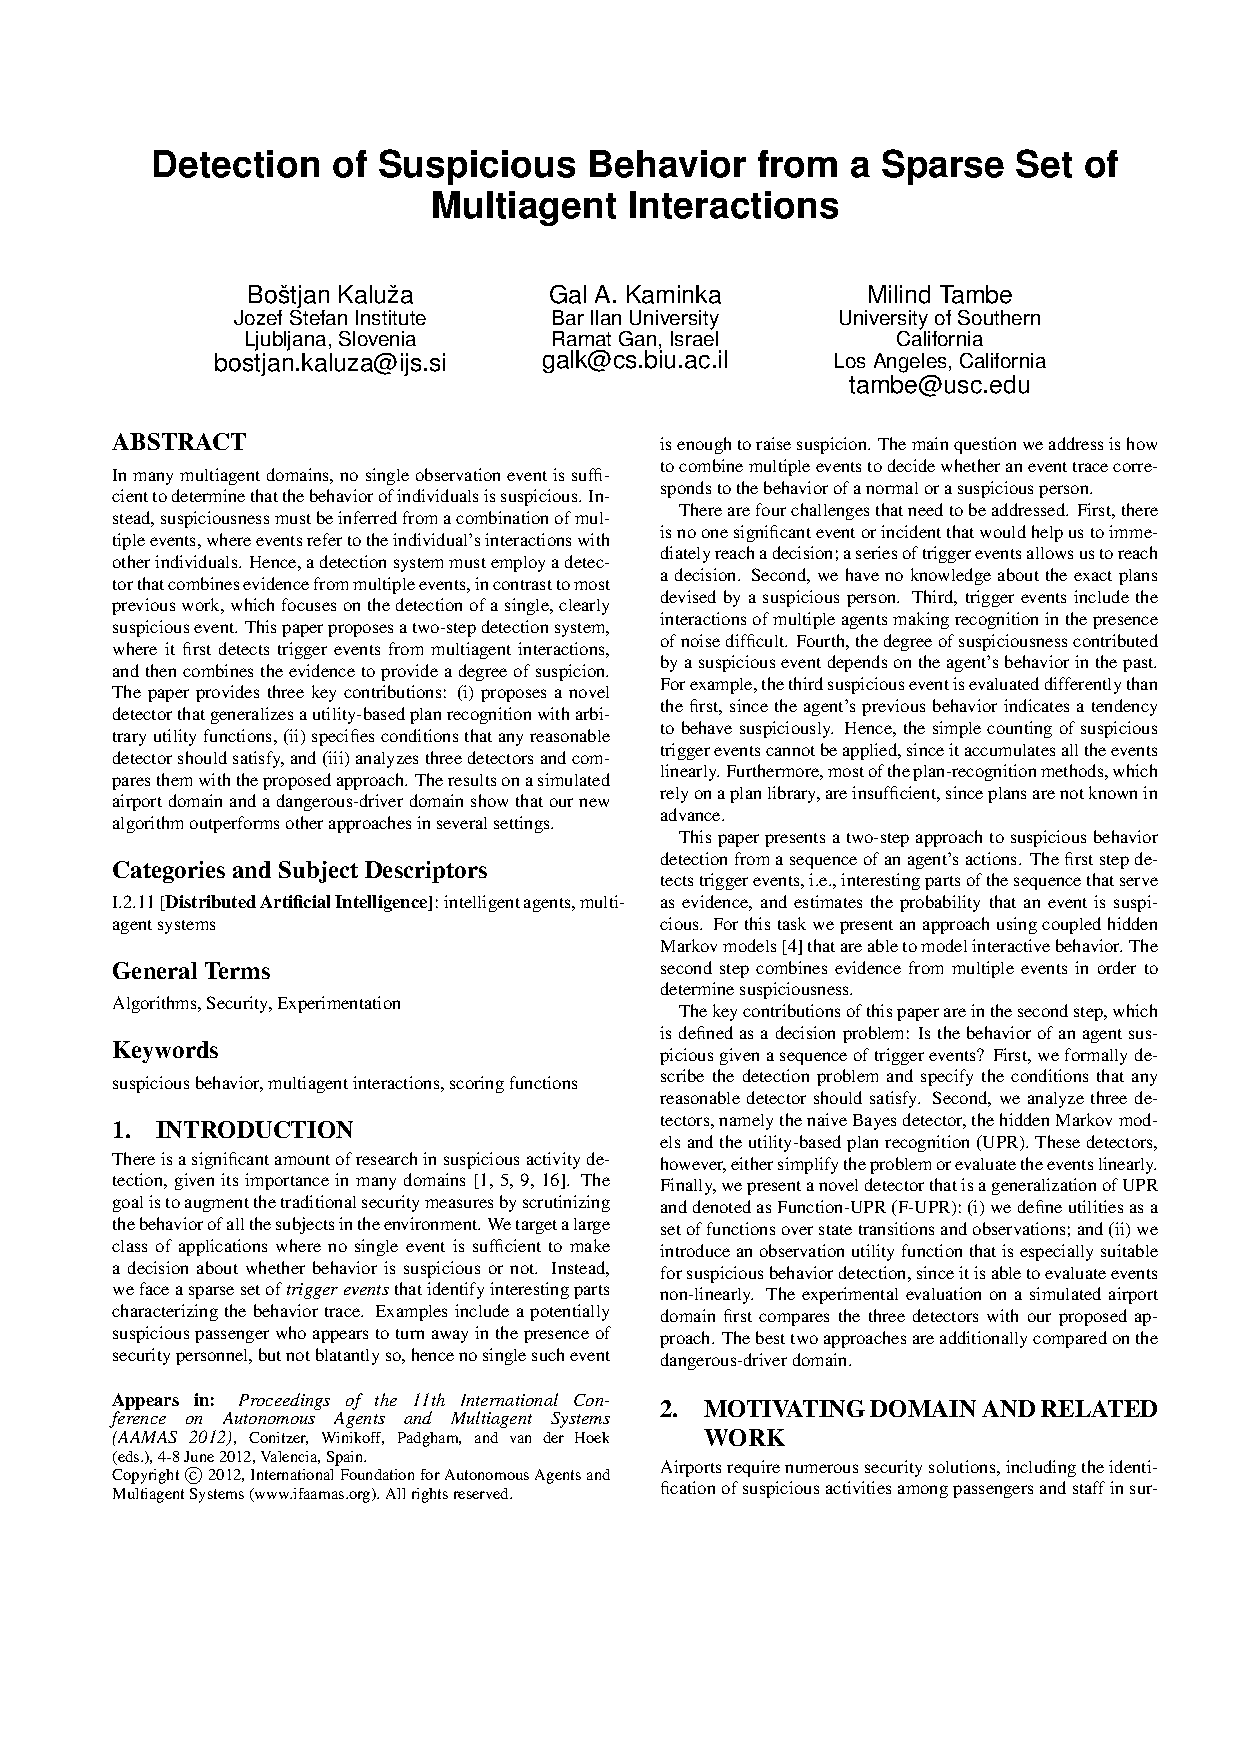
\includepdf[pages=1-last, fitpaper=true, addtotoc={
% 1, section, 1, {Detection of Suspicious Behavior from a Sparse Set of Multiagent Interactions}, sec:aamas, %
% 1, subsection, 2, {Introduction}, sec:aamas:intro, %
% 1, subsection, 2, {Motivating Domain and Related Work}, sec:aamas:related, %
% 2, subsection, 2, {Definitions and Assumptions}, sec:aamas:definitions, %
% 3, subsection, 2, {Problem Definition}, sec:aamas:problem, %
% 4, subsection, 2, {Detectors}, sec:aamas:detectors, %
% 	4, subsubsection, 3, {Naive Bayes Detector}, sec:aamas:detectors:bayes, %
% 	4, subsubsection, 3, {Hidden Markov Models}, sec:aamas:detectors:hmms, %
% 	5, subsubsection, 3, {Utility-Based Plan Recognition}, sec:aamas:detectors:upr, %
% 	%5, subsubsubsection, 4, {Utilities as Potential Functions}, sec:aamas:detectors:upr:potential, %
% 	%5, subsubsubsection, 4, {Observation Utility for Suspicious Behavior Detection}, sec:aamas:detectors:upr:exponential, %
% 6, subsection, 2, {Experimental Evaluation}, sec:aamas:experiments, %
% 	6, subsubsection, 3, {Airport Domain}, sec:aamas:experiments:airport, %
% 	8, subsubsection, 3, {Catching a Dangerous Driver}, sec:aamas:experiments:driver, %
% 8, subsection, 2, {Conclusion}, sec:aamas:conclusion, %
% 8, subsection, 2, {References}, sec:aamas:references %
% }]{article/AAMAS2012.pdf}

This chapter focuses on two applications in surveillance domain, where the goal is to detect suspicious agents in the environment. In particular, the chapter targets a large applications class where no single event is sufficient to gauge whether or not agent behavior is suspicious. Instead, we face a sparse set of \emph{trigger events} that identify interesting parts in behavior trace. The first application considers suspicious passenger detection at an airport, while the second application tackles dangerous driver detection.
%The main tasks are, hence, first to detect trigger events, and then combine them over time into a reliable behavior evaluation.


\section{Introduction and Background}


There is significant suspicious activity detection research, given its importance in many domains~\citep{Arsic, Duong2005, Helman1993, Vaswani}. The goal is to augment the traditional security measures by scrutinizing the all subjects' behavior in the environment. 
%
%We target a large class of applications where no single event is sufficient to make a decision about whether behavior is suspicious or not. Instead, we face a sparse set of \emph{trigger events} that identify interesting parts characterizing the behavior trace.  %Examples include a suspicious passenger at an airport that immediately flees the area when noticed by security or a reckless driver zigzagging across two lanes. 
%Examples include a potentially suspicious passenger who appears to turn away in the presence of security personnel, but not blatantly so, hence no single such event is enough to raise suspicion.
The main question we address is how to combine multiple events to decide whether an event trace corresponds to the behavior of a normal or a suspicious person. 





%There are four challenges that need to be addressed. 
%First, there is no one significant event or incident that would help us to immediately reach a decision; a series of trigger events allows us to reach a decision. Second, we have no knowledge about the exact plans devised by a suspicious person. Third, trigger events include the interactions of multiple agents making recognition in the presence of noise difficult. 
%Fourth, the degree of suspiciousness contributed by a suspicious event depends on the agent's behavior in the past. For example, the third suspicious event is evaluated differently than the first, since the agent's previous behavior indicates a tendency to behave suspiciously. 
%Hence, the simple counting of suspicious trigger events cannot be applied, since it accumulates all the events linearly. Furthermore, most of the plan-recognition methods, which rely on a plan library, are insufficient, since plans are not known in advance.


In the airport scenario, various systems were introduced to automatically detect some of the threats, such as leaving objects behind~\citep{Hongeng2003}, suspicious trajectory paths~\citep{Vaswani}, 
%suspicious transportations~\cite{Arsic},  
thefts~\citep{Hongeng2003}, and vandalism acts and fights~\citep{AdvisorProject}. 
There is also a commercially available system~\citep{IBMsmart} that is able to detect such events as running passengers, climbing over a fence, etc.  
However, these approaches mainly deal with the detecting single, clearly suspicious incidents and do not address accumulating suspicion.


%BACKUP PARA: There are four challenges that need to be addressed. First, there is no significant event or incident that would help us to immediately reach a decision; a series of trigger events over time establishes our decision with accumulating effect. This would normally do for the use of plan recognition methods, but unfortunately, the second challenge is that we have no knowledge about the exact plans devised by a suspicious person. Thus most of the plan recognition methods, which rely on a plan library, are insufficient. Third, trigger events include interactions of multiple agents making recognition under noise difficult. Fourth, evaluation of an event changes degree of suspiciousness with the number of detected suspicious events in the past; that is, two suspicious events are evaluated differently according to individual's behavior in the past. Hence, simple counting of suspicious trigger events cannot be applied, since it accumulates all events linearly.



%These challenges disallow direct application of plan recognition as they assume that the plan library is known in advance. Furthermore, simple counting of suspicious trigger events disallows non-linear accumulation. 
%assigned degree of suspiciousness
%The main question we are addressing is how to decide whether an event trace corresponds to behavior of a normal or a suspicious agent.
%interesting parts from \emph{trigger events}, that is interesting events that help to establish our decision. 
%TODO: UPDATE. The current approaches can be divided into three groups. The first group focuses on significant events, we call them incidents, that are used as the evidence of suspicious behavior (for example, leaving object behind [?], vandalism acts[], running passengers[]). Second, trajectory-based approaches examine trajectory shape to identify suspiciousness.  

%The main question we are addressing is how to decide whether an event trace corresponds to behavior of a normal or a suspicious agent. Standard approaches include modeling both normal and suspicious behavior traces of a single agent using probabilistic models, plan recognition, etc. However, behavior of an agent in a multiagent environment is influenced by other agents, which is usually not captured in such models. Instead, we focus on \emph{trigger events} that identify interesting parts characterizing the behavior trace. Trigger events can present either positive or negative belief about the motivating goal and tend to be noisy; it is not clear if a person emitting suspicious events is indeed acting suspiciously. They also involve interactions of multiple agents making recognition under noise difficult. In many cases no single action or event is sufficient to reveal adversary intentions, but a collection of events enables the observer to infer the underlying intentions. Moreover, our belief that an individual is acting suspiciously  increases with the number of detected suspicious events non-linearly; that is, individual's behavior in the past affects current evaluation.


%Problems with current approaches\\
% - modeling complete behavior traces is not feasible\\
% - we establish a formal framework for evaluating event traces and show where are the problems
% - it is hard to do take history into account\\

%Our solution\\
% - focuses on trigger events\\
% - heuristic approach
% - defines a family of \emph{well-behaved} evaluation functions\\
% - proposes an instance of function\\
This chapter addresses how to instantiate the unified detection framework to detect trigger events, that is, interesting trace parts  that serve as evidence, and combine evidence from multiple events in order to estimate suspicion. 
%The first task is based on an approach using coupled hidden Markov models~\cite{Brand} that are able to model interactive behavior. The second task combines evidence from multiple events in order to determine suspiciousness.
%
%The key contributions of this paper are in the second step, which is defined as a decision problem: {Is the behavior of an agent suspicious given a sequence of trigger events?} First, we formally describe the detection problem and specify the conditions that any reasonable detector should satisfy. Second, we analyze three detectors, namely the na{\"i}ve Bayes detector, the hidden Markov models and the utility-based plan recognition (UPR). These detectors, however, either simplify the problem or evaluate the events linearly. Finally, we present a novel detector that is a generalization of UPR and denoted as Function-UPR (F-UPR): (i) we define utilities as a set of functions over state transitions and observations; and (ii) we introduce an observation utility function that is especially suitable for suspicious behavior detection, since it is able to evaluate events non-linearly.
%
The experimental evaluation of a simulated airport application first compares the three detectors from Chapter \ref{chap:accumulation} (Section~\ref{sec:acc-detectors}) with our proposed approach (Section~\ref{sec:FUPR}). The best two approaches are additionally compared in the dangerous-driver application.

%The experimental evaluation on a simulated airport domain first compares the three detectors with our proposed approach. We also compare it to an approach that uses a complete sequence of actions (instead of a sequence of trigger events). \hl{Finally, the best two approaches are compared on the dangerous-driver domain}.


%The experiments in a simulated multiagent environment show that the proposed approach outperforms other approaches in several settings. 
%UPR and its generalization F-UPR are finally compared on the dangerous driver domain confirming the results.


% and assigns them probabilities that  formally defines the problem within a Bayesian framework, analyzes four algorithms to address it, and introduces a new algorithm able to address the abovementioned challenges.
%
%
%This paper introduces a Bayesian plan recognition framework as a formal definition of the problem, analyses four detectors and introduces a new detector that addresses the above-mentioned challenges. 
%The paper introduces three key contributions. 
%First, we show the optimal detection within the proposed Bayesian framework and discuss why it is not feasible in practice. Next, we introduce a Na{\" i}ve Bayes approximation as well as two detectors, namely Hidden Markov Models [] and Utility Plan Recognizer []. Unfortunately, these detectors either over-simplify the approximation, do not take into account history, and accumulate evaluation linearly. Finally, we introduce a family of \emph{scoring functions} for evaluating event traces and propose a heuristic function that evaluates an event trace non-linearly. 
%Experimental results in a simulated airport domain 

%The key contributions of this paper are (1) introduction of a Bayesian suspicious detection framework, (2) analysis of four detectors

%five algorithms. The It shows that the optimal detector within Bayesion framework  solution whithin for evaluating event traces and evaluation (that is, whether a trace is produced by a suspicious agent) does take into account interactions between events. More precisely, evaluation of an event depends not only on the current time step but also on the events in prior time steps. 
%We propose a heuristic approach that defines a family of \emph{well-behaved} scoring functions that interpret an event trace to produce a score presenting overall suspicion that the trace corresponds to the behavior of a suspicious agent. The key component is that the events are evaluated according to the behavior of the agent in the past. We present a set of scoring functions that satisfy that conditions.


%Verification procedure\\
% - evaluation on motivating domain -- airport scenario\\
% - proposes event detection procedure\\
% - compare different approaches using simulation
%Experimental evaluation on a simulated airport domain first compares the three detectors with our proposed approach. We also compare it to an approach that uses a complete sequence of actions (instead of a sequence of trigger events). The experiments in a simulated multiagent environment show that the proposed approach outperforms other approaches in several settings.






%%%%%%%%%%%%%%%%%%%%%%%%%%%%%%%%%%%%%%%%%%%%%%%%%%%%%%%%%%%%%%%%%%%%%%%%%%%%%%%%%%%%%%%%%%%


% \section{Related Work}
% \label{sec:domain}
% %A dramatic increase in air travel in recent years has made every airport a potential terror target, hence intense security is a necessary requirement. This global transportation system is no longer considered as safe, but rather as a potential liability exposed to terrorist attacks and other criminal activities, such as drug and contraband trafficking. Airports require vast security solutions including the identification of suspicious activities amongst passengers and staff in surrounding areas.
% \noindent 
% Airports require numerous security solutions, including the identification of suspicious activities among passengers and staff in surrounding areas.
% %
% Our goal is to monitor passengers during the time they spend at the airport and to detect those that indicate a high level of stress, fear or deception. It is reasonable to assume that there is a camera network to track a passenger throughout the airport. We focus on a task where no single event is sufficient to identify a suspicious passenger, but a series of events establishes the decision over time. The detection of events might be limited due to noise or an inability to extract some features (for example, using a ceiling-mounted camera one can extract the trajectory of a passenger, but not facial expressions), hence a normal person may appear suspicious (and vice versa).
% Also, a precise plan of the suspicious passenger is not known in advance. 
% %
% %Observer might be limited due to various reasons such as inability to detect characterizing features and noisy trigger-event detectors.
% %
% Other domains of interest may include identifying a reckless driver executing dangerous (but still legal) maneuvers~\cite{Avrahami-Zilberbrand2009}, detecting a pirate vessel that plans to capture a transport vessel and therefore avoids security patrols, etc. 

%To run proof-of-concept tests we consider a simulated environment due to several reasons. First, a simulation is controllable and repeatable in terms of ensuring statistical relevance. Second, obtaining real-world data with annotated suspicious behavior might present a difficulty in terms of cost and amount of data required to create a statistically representative dataset. In practice there are tens of hours of several hundred people with only a few instances of suspicious behaviors. Third, a simulator enables the control of the amount of noise that is otherwise introduced by various vision systems (occlusions, false detections, etc.). And last, real-world data in security domain present a difficulty due to privacy issues, confidentiality and national security concerns.

%To run proof-of-concept tests we consider a simulated environment, mainly to avoid difficulties due to privacy and confidentiality issues and as well as due to absence of annotated suspicious behavior in real world. A simulator also enables to control the amount of noise otherwise introduced by various vision systems (occlusions, false detections, etc.), and provides  controllable and repeatable situations. Experiments in this paper use ESCAPES~\shortcite{Tsai2011}, a state-of-the-art multiagent simulator for airport evacuations with several types of agents exhibiting behaviors of regular travelers, authorities, and families. We assume that behavior of the agents corresponds to the behavior of real passengers at the airport.

%
%ESCAPES consists of two parts, a 2D environment based on the open-source project OpenSteer~\cite{OpenSteer}, outputting agents' physical and behavioral information into files, and a 3D visualization component using the Massive Software~\cite{Massive}. 
%The first part consists of agents interacting in an environment, outputting their physical and behavioral information into files later used in a customized Massive extensions to generate 3D movies of the scenarios.
%In one scenario, they modeled the Tom Bradley International Terminal at Los Angeles International Airport including terminals and shops as a realistic simulation environment. This served as our playground for introducing suspicious behaviors prior to an evacuation occurring.


%In many cases, the extra scrutiny is a casual conversation with a TSA behavior officer that shows someone is innocent, 

%"behavioral surveillance" has "enormous potential for violating" privacy.

%"The shortcoming is, we don't know how many people are showing suspicious behaviors and aren't being noticed," Ekman said.

%Although observers can perceive whether someone appears anxious or is acting deceptively, they can't tell whether that person is planning an attack or something such as an extramarital affair, Levenson said.

%Our goal is to monitor a passenger 

%Airport security has increased drastically in recent years.
%Nowadays the security at the airports 
%Motivation...



%\section{Related Work}
%\label{sec:RelatedWork}


%An approach for monitoring behavior of passengers over longer periods of time relies upon security personnel such as behavior detection officers (BDOs) that patrol airport to identify passengers who display \emph{involuntary physical and physiological actions} (US Transportation Security Administration (www.tsa.gov) trained and deployed BDO officers at 161 US airports). In this context we strive to observe passengers for the whole time they spend at the airport. We are focused on trigger events in terms of actions, events and incidents that can be potentially suspicious in order to identify individuals who exhibit behaviors that indicate high levels of stress, fear or deception.

%Describe differen t approaches
%\noindent
%There are two approaches to detecting deviant behavior~\cite{Avrahami-Zilberbrand2009}: \emph{suspicious} and \emph{anomalous} behavior detection. The first approach assumes a behavior library that encodes \emph{negative behavior}, and thus recognizing observed behavior corresponds to identifying a match in the library. The second approach uses the behavior library in an inverse fashion, meaning that the library encodes only \emph{positive behavior}. When an observed behavior cannot be matched against the library it is considered as anomalous. Several approaches have been proposed to tackle the problem either way. % and the literature is vast. 
% In the airport scenario various systems were introduced to automatically detect some of the threats, such as leaving objects behind~\cite{Hongeng2003}, suspicious trajectory paths~\cite{Vaswani}, 
% %suspicious transportations~\cite{Arsic},  
% thefts~\cite{Hongeng2003}, and vandalism acts and fights~\cite{AdvisorProject}. 
% There is also a commercially available system~\cite{IBMsmart} that is able to detect events such as running passengers, climbing over a fence, etc.  
% However, these approaches mainly deal with the detection of single incidents, which are clearly suspicious. They do not address accumulating suspicion as we do.
% % or monitor only a part of the premises. 

% %We focus to related research within recognition from multiple events emphasasing  probabilistic models and plan recognition. 
% Another area of related work includes hidden Markov models (HMMs)~\cite{Rabiner1989} that are widely used in traditional activity recognition for modeling a sequence of actions.  Brand et al.~\cite{Brand} introduced coupled HMMs as an extension with multiple hidden interacting chains that are able to model interactive behavior. 
% %Moreover, layered HMMs~\cite{Oliver2004} and hierarchical HMMs~\cite{Fine1998} can handle activities that have hierarchical structure, for example, activity recognition from trajectories \cite{Nguyen2005}. 
% Duong et al.~\cite{Duong2005} focused on the duration of activities and introduced switching hidden semi-Markov models that provide probabilistic constraints over the duration of plans, and applied them to the detection of anomalies in the activities of daily living. 
% %Vaswani et al.~\cite{Vaswani} introduced Continuous State HMMs for modeling trajectories in order to detect anomalous activities. 
% Although widely used, HMMs may become inadequate when actions are more complex or have long-term temporal dependencies~\cite{KollerFriedman2009}. 
% %
% %Even though our approach is completely different from HMMs, we further discuss some variations of HMMs in Section~\ref{sec:Experiments}.% and compare them with ESPY.


% %\subsection{Utility-based Plan Recognition}
% %\label{sec:UPR}
% Plan recognition algorithms may use a hybrid approach for suspicious activity recognition. A symbolic plan recognizer is used to filter consistent hypotheses, passing them to an evaluation engine, which focuses on ranking. Geib and Goldman presented PHATT~\cite{Geib2009}, a probabilistic approach based on tree grammars able to cope with interleaved goals, partially ordered plans, and failed observed actions. Sukthankar and Sycara~\cite{Sukthankar-AAAI2008} addressed plan recognition for multiagent teams, where plans were ordered by linear accumulation of observed actions consistent with the plan.
% Another approach is presented by Avrahami-Zilberbrand and Kaminka~\ref{Avrahami-Zilberbrand2009, Avrahami-Zilberbrand2007}. Utility-based Plan Recognition (UPR) introduces utility to the observer in selecting the recognition hypotheses. The main strength of UPR is that it can incorporate an observer's bias to events with a low likelihood, for example, the a-priori probability for planting a bomb is very low, but detecting it has a high expected utility. We further discuss this approach in Section~\ref{sec:UPR}. 
% %Other approaches based only on symbolic plan recognition This would normally do for the use of plan recognition methods, but unfortunately, the second challenge is that we have no knowledge about the exact plans devised by a suspicious person.

% Furthermore, intrusion detection systems analyze a variety of person activities to identify suspicious computer activities. Helman and Liepins~\cite{Helman1993} proposed an intrusion detection system that provides a rating for computer activities, demonstrating frequency estimator and matching rules. Esponda et al.~\cite{Esponda2004} analyzed tradeoffs between positive and negative activity patterns in the library and presented an approach based on partially matching rules. These approaches similarly address the problem of how to decide whether a person's activity is suspicious, but differ significantly in using a different approach to match and assess behavior. 

%Our approach in a similar way evaluates the events using utilities but with two key differences: (i) utility functions dynamically change in order to adapt to the behavior history of the observed agent; and (ii) evaluation process in ESPY introduces the forgetting mechanism in order to deal with noise.




%%%%%%%%%%%%%%%%%%%%%%%%%%%%%%%%%%%%%%%%%%%%%%%%%%%%%%%%%%%%%%%%%%%%%%%%%%%%%%%%%%%%%%%%%%%

% \section{Definitions and Assumptions}
% \label{sec:definitions}
% \noindent
% Our methods are general, but for illustrative purposes we will make use of the airport domain to provide examples. We treat subjects as agents in a multi-agent environment. At this point we assume that we can perfectly observe their actions. 
% \begin{definition}
% 	\emph{Action} $a_t$ is a tuple of observed feature values\\ $\langle f_1, ..., f_n \rangle$ that describe state of an agent at a given time stamp $t$.
% \end{definition}
% %
% \begin{definition}
% 	\emph{Action trace} $\avec{l}$ is a totally-ordered sequence of $l$ actions $\avec{l}=(a_1,a_2,...,a_l)$.
% \end{definition}
% %
% \begin{definition}
% 	\emph{Trigger event} $x^{i,j}=(a_i, ..., a_j)$ is a subsequence of action trace $\avec{k}$ (s.t.\  $1 \leq i < j \leq k$). A trigger event $x$ is described by probabilities that the corresponding subsequence is suspicious $s(x)$ and normal $n(x)$.
% \end{definition}
% %
% \begin{definition}
% 	\emph{Event trace} $\xvec{k}$ is a totally-ordered sequence of $k$ trigger events $\xvec{k}=(x_1,x_2,...,x_k)$.
% \end{definition}

% We address the problem of suspicious behavior detection in two steps, as shown in Figure~\ref{fig:architecture}. The first step analyzes an action trace and the surrounding environment to detect trigger events that characterize its interesting parts. The event trace then enters the second step, where it is evaluated. If the evaluation result exceeds a threshold value or is large relative to other evaluations of the event traces, then it is considered as suspicious.

% \begin{figure}[!ht]
% \centering
% 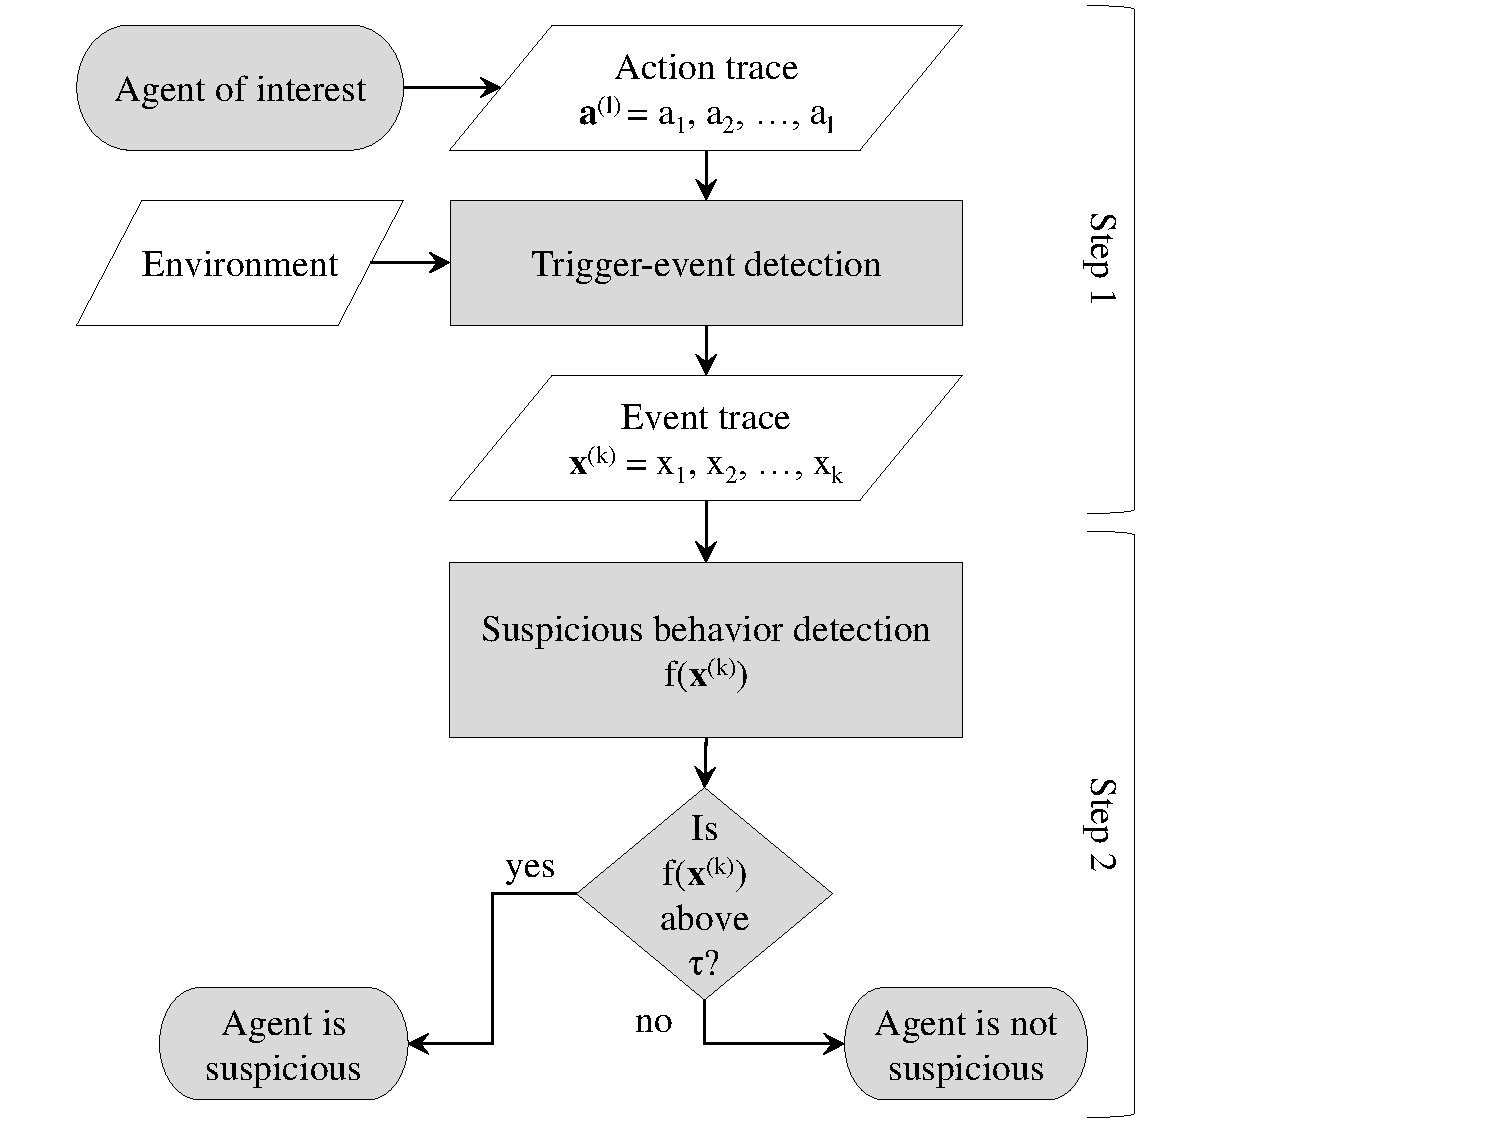
\includegraphics[width=0.7\linewidth, bb=34 10 523 530]{chap_surveillance/flowchart.pdf}
% \caption{Two-step detection of suspicious behavior: (1) detection of trigger events and (2) detection of suspicious behavior.}
% \label{fig:architecture}
% \end{figure}


% %\subsection{Trigger Events}
% %\label{sec:events}
% %\noindent
% Trigger events can be any kind of partial observations we are able to extract from the domain. In the airport domain, one can focus on people exhibiting indications of suspicious behavior, such as taking photos of critical infrastructure, revisiting the same location, evading the area when noticed, standing in customer service but not requesting the service, etc. 
% %We focus on a rather novel descriptor we were unable to find in the literature on suspicious behavior detection at the airport. 
% We focus on a well-known detector obtained from conversations with domain experts. %and commonly used by behavior detections officers\footnote{An approach for monitoring behavior of passengers over longer periods of time relies upon security personnel such as behavior detection officers (BDOs) that patrol airport to identify passengers who display \emph{involuntary physical and physiological actions}. US Transportation Security Administration (www.tsa.gov) trained and deployed BDO officers at 161 US airports.}.
% We observe the interactions between agents at the airport, more precisely, we are interested in how a passenger behaves in the presence of a uniformed authority figure. A person exposed to a high level of stress produces behavior that indicates fear, anxiety, pressure, tension, deception, etc. Hence, it is rational for the suspicious agent to minimize contacts with the authorities. Note, that no single avoidance is enough to raise a flag, but many such events put together cause the person to be treated as suspicious. 

% %This results in a set of partial observations describing interactive behavior of a passenger. The recognition process first extracts all interactions between passengers and authority figures inside a given radius, producing a set of trajectory pairs that are transformed to relative presentation. 

% A trigger-event detection able to identify interactive behavior may rely on coupled hidden Markov models (CHMMs), which are briefly described below. The reader is referred to~\cite{Brand} for details; the CHMMs are not the main contribution of the paper.
% %To differentiate between authority-regular and authority-suspicious interactions we present an approach based on coupled hidden Markov models (CHMM). 
% %
% The observations consist of two action traces, namely the action trace of the agent of interest and the action trace of an authority agent when they are within some predefined radius. The CHMMs are able to model the complex, interactive behavior by two HMM chains, where the hidden states from one chain directly impact on the hidden states from the other chain. Figure~\ref{fig:CHMMs} illustrates the CHMM for a pair of action traces with length $l=3$. The current state $Q_t^A$ of agent $A$ is affected by both its previous state $Q_{t-1}^A$ and previous state $Q_{t-1}^B$ of the agent $B$ (similarly $Q_t^B$ is affected by $Q_{t-1}^B$ and $Q_{t-1}^A$). Each state $Q_i$ also impacts the corresponding observation state $Y_t$. For example, if the authority agent moves toward the suspicious agent, the next state of the latter takes this into account and produces an action for an avoidance maneuver. 
% %The joint distribution for a pair of traces of length $k$ can be obtained by unrolling the network until we have $k$ slices, and them multiplying together all of the conditional probability distributions. 


% \begin{figure}[!ht]
% \centering
% 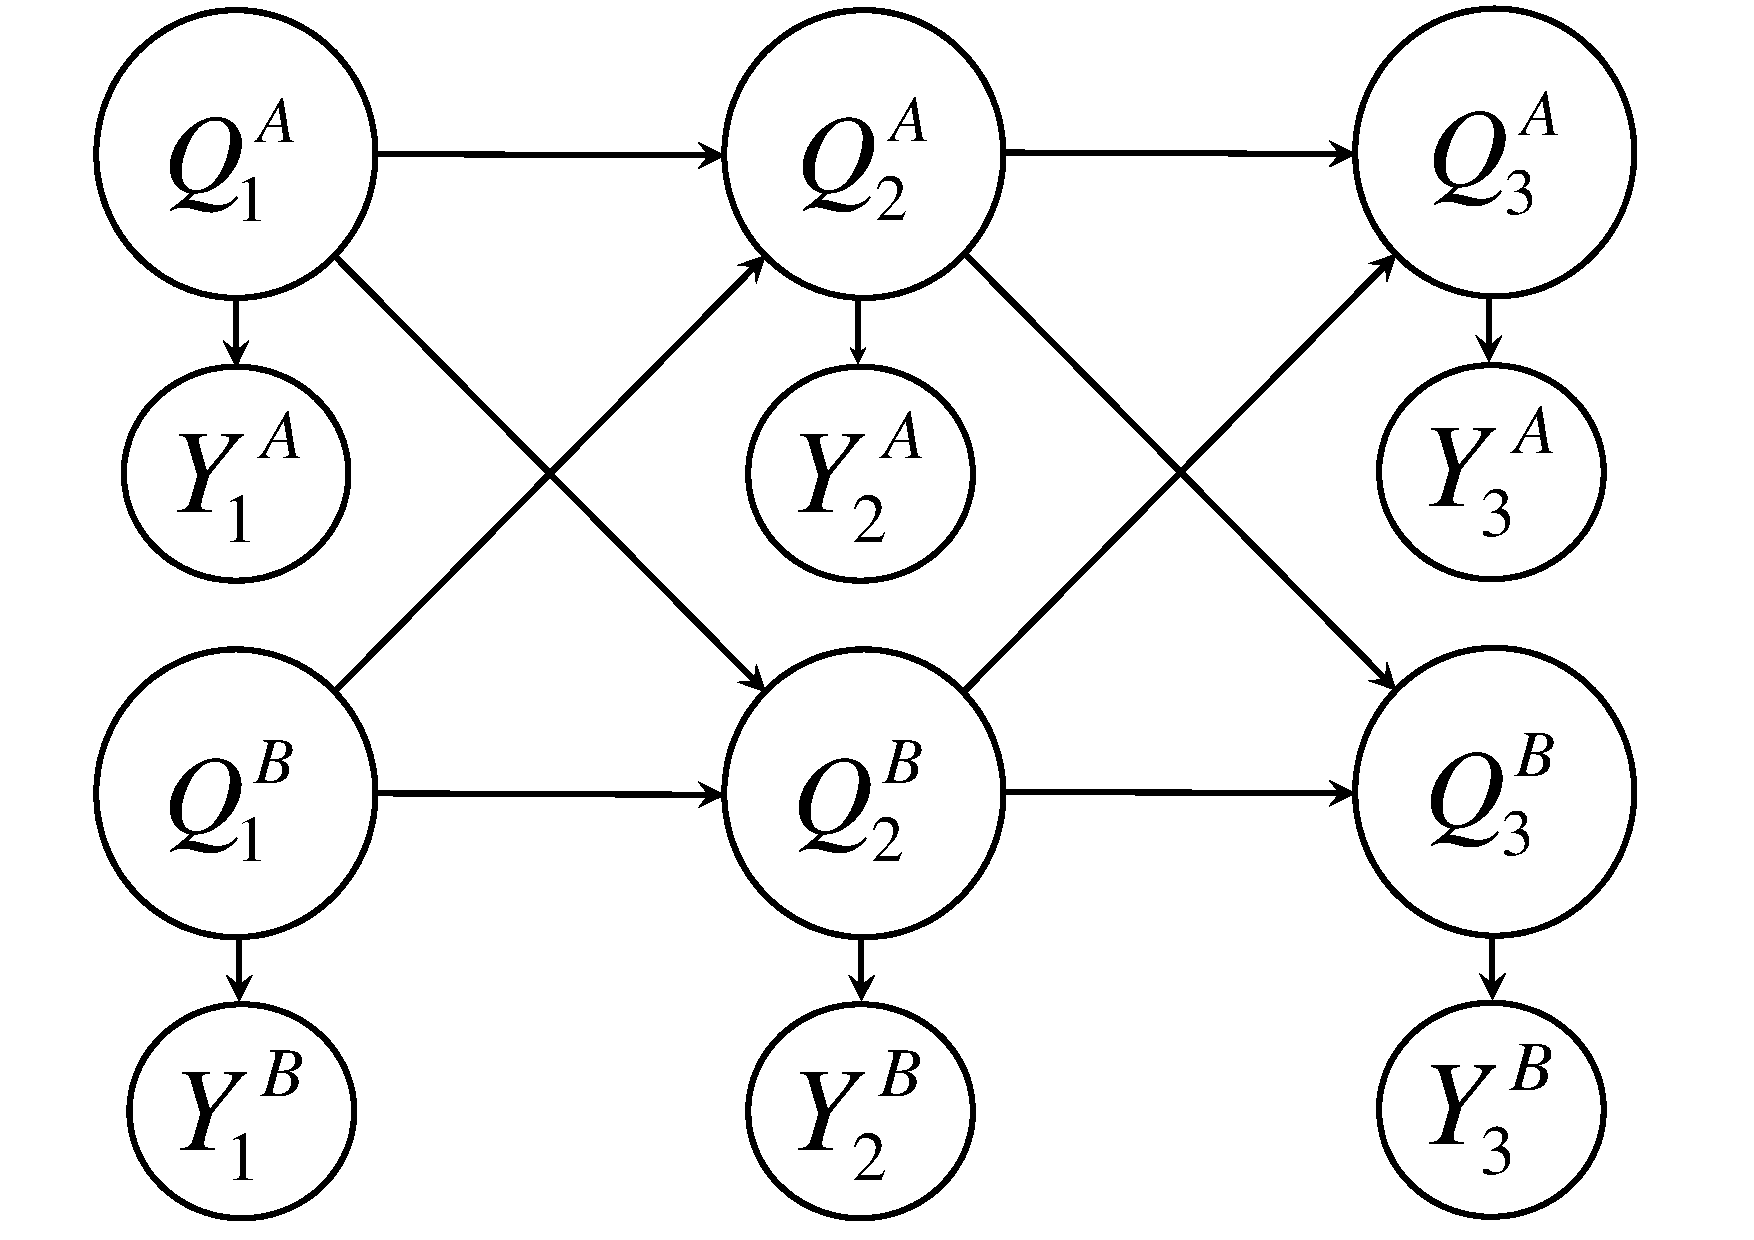
\includegraphics[bb=0 0 595 830, angle=-90, width=0.5\linewidth]{chap_surveillance/chmm.pdf}
% \caption{An example of CHMM for a pair of action traces with length $l=3$.}
% \label{fig:CHMMs}
% \end{figure}

% A regular passenger may not turn or do anything different in the presence of authorities, while a suspicious person will (although as described below, an observer may not have perfect observability). Therefore, we create and train two CHMMs: $\hat{N}_I$ models the interactions produced by authorities and regular passengers, while $\hat{S}_I$ models the interactions produced by authorities and suspicious passengers. For a new event (interaction) $x$ we compute the posterior probability that the event is generated with both models yielding $\hat{n}_I(x)=\Prob\{x|\hat{N}\}$ and $\hat{s}_I(x)=\Prob\{x|\hat{S}\}$, respectively. %We also experimented with more complex CHMM structures including other features such as relative speed and distance, but the results were comparable or even worse.


% %As a trigger event we also extract all turns in absence of authority when the trajectory curvature exceeds a threshold value. Probabilities that a turn event was generated by suspicious $\hat{n}_T(x)$ or regular passenger $\hat{s}_T(x)$ is acquired with frequentist estimator from the learning set $D_l$.
% %
% %
% %The second architecture (Figure~\ref{fig:CHMM-3}) incorporates additional information in the form of a model of relative speed between two agents. This model directly impacts the states of both agents. The idea behind this architecture is to improve recognition results with an additional information.
% %
% %Note that for an interaction of length $T$ the architectures presented in Figure~\ref{fig:CHMMs} are unrolled to $T$ slices. %(similar as in Figure~\ref{fig:HMM-4}). 


% %\begin{figure}[!ht]
% %\centering
% %\subfigure[]{
% %\includegraphics[width=0.25\linewidth]{CHMM-2}
% %\label{fig:CHMM-2}
% %}
% %\subfigure[]{
% %\includegraphics[width=0.25\linewidth]{CHMM-3}
% %\label{fig:CHMM-3}
% %}
% %\caption{CHMM presented as 2-sliced DBN: (a) modeling actions of two agents and (b) modeling both actions and relative speed.}
% %\label{fig:CHMMs}
% %\end{figure}




% %%%%%%%%%%%%%%%%%%%%%%%%%%%%%%%%%%%%%%%%%%%%%%%%%%%%%%%%%%%%%%%%%%%%%%%%%%%%%%%%%%%%%%%%%%%


% \section{Problem Definition}
% \label{sec:problem}
% \noindent
% This section formally analyzes how to evaluate a sequence of trigger events. We leverage the Bayesian framework for intrusion detection~\cite{Helman1993} for the problem definition.
% At each time step $t$ we observe an event $x_t$, generated by a hidden stochastic process $H$. Now suppose that $H$ is a mixture of two auxiliary stochastic processes, namely the normal process $N$ and the suspicious process $S$ that correspond to a normal and a suspicious passenger. The random variable $y_t=0$ if $x_t$ is generated by $N$ and $y_t=1$ if $x_t$ is generated by $S$. Since a suspicious passenger always emits a suspicious event (and a normal person a normal event), $y$ for a specific agent does not change over time. In reality, there can be many subprocesses contributing to each of $N$ and $S$; that is, many normal persons with different behavior patterns; however, here we assume only a single $N$ and a single $S$ that capture all the variability. 

% To this point we assumed that an observer is able to perfectly observe whether an event is generated by $S$ or $N$. In practice, however, it may appear that a normal person emits suspicious events (or vice-versa). An observer might be limited for various reasons, such as an inability to detect characterizing features and noisy trigger-event detectors. Therefore, we relax this assumption as follows. An event $x_t$ is observed as generated by $N$ with the probability $n(x_t) = \Prob\{H(t)=x_t|y_t=0\}$ and as generated by $S$ with the probability $s(x_t) = \Prob\{H(t)=x_t|y_t=1\}= 1 - n(x_t)$. The mixture distribution of an event $x_t$ and a prior probability $\lambda$ is
% \begin{equation}
%   \Prob\{H(t)=x_t\} = \lambda s(x_t) + (1-\lambda) n(x_t).
% \end{equation}
  

% The objective of suspicious behavior detection is to identify those traces $\xvec{k}=(x_1,x_2,...,x_k)$ that are likely to be suspicious activities; that is, traces $\mathbf{x}$ for which
% \begin{equation}
% \label{eq:detect}
% 		%\Prob\{y_t=1|H(t)=x_t, t=1,...,k\} > \tau,
% 		\Prob\{y=1|H(t)=x_t, t=1,...,k\} > \tau,
% \end{equation}
% is above some threshold $\tau$ or is large relative to the probability for other traces.
% %
% %An event $x_t$ may depend on the current step $t$ as well as on the pattern of events generated at time steps prior $t$. 
% %This allows that $H$ is non-stationary, where its distribution depends both on actual time step $t$ and previously observed events, for example, if the observer identifies three out of four events in an event trace as generated by $N$, a new event will be most likely again observed as generated by $N$. 
% %The non-stationary nature might reflect that: (i) agent behavior depends on his/her prior actions; (ii) agent's executing goals change over time; (iii) behavior changes over time (different population of agents); and (iv) the environment changes over time.

% The reason why this problem is difficult is because of the non-linear effect. Consider the following example. Suppose we observe a person do a U-turn in front of a police officer, so that the likelihood that this was a suspicious person becomes high. Later we see the same person doing a half-turn in front of a police officer. This trigger event if seen on its own, would not contribute much to the overall suspicion. However, following the initial turn we had observed, this new turn is a much stronger evidence to be attributed to the overall suspicion, because we bias the new event with our previous observation.

% Theoretically, it might be possible to optimally detect suspicious behavior using Equation~(\ref{eq:detect}). Unfortunately, this is usually not the case in practice. 
% %
% %TODO: why is this difficult? Why not use existing methods?
% %
% To see this, let us assume a prior probability $\lambda=\Prob\{y_t=1, t=1, ..., k\}$. In most cases $\lambda$ is close to $0$, since in real-world applications suspicious activities are rare. 
% %
% Let the stochastic processes $N$, $S$ and $H$ denote $n(\xvec{k})=\Prob\{H(t)=x_t, t=1, ..., k|y=0\}$, ~~$s(\xvec{k})=\Prob\{H(t)=x_t, t=1, ..., k|y=1\}$, ~and~~ $h(\xvec{k}) = \Prob\{H(t)=x_t, t=1, ..., k\}$, respectively.
% Using Bayes theorem we can derive from Equation~(\ref{eq:detect})
% \begin{eqnarray}
% \label{eq:bayes}
%         \lefteqn {\Prob\{y=1|H(t)=x_t, t=1,...,k\} = \frac{\lambda \cdot s(\xvec{k})}{h(\xvec{k})} = } \\
% 		%&&=\frac{\Prob\{y_t=1, t=1, ..., k\} \cdot \Prob\{H(t)=x_t|y_t=1, t=1,...,k\}}{\Prob\{H(t)=x_t|t=1,...,k\}} \nonumber\\
% 		%&&=\frac{\lambda \cdot s(\xvec{k})}{h(\xvec{k})} =\nonumber\\
% 		&&=\frac{\lambda \cdot \prod_{t=1}^k s(x_t|x_i, _{i=t-1,...,1})}{\lambda \prod_{t=1}^k  s(x_t|x_i, _{i=t-1,...,1}) + (1-\lambda) \prod_{t=1}^k  n(x_t|x_i, _{i=t-1,...,1})} \nonumber
% \end{eqnarray}

% To this point we implicitly assumed that the distributions $\lambda$, $n$ and $s$ are reliably estimable. The degree to which this assumption is valid depends on our detection capability.
% %
% %For each trace $tr_j=\{x_1,...,x_n\}, tr_j \in D_l$ we have a corresponding trace $Y_j=\{y_1, ..., y_n\}$ that specifies whether events were generated by normal or suspicious agent, meaning $y_1=y_2=...=y_n$. 
% Suppose we have a sufficiently large dataset $D_l$ of labeled event traces, we can estimate the prior probability $\lambda$ from the $D_l$ using the relative frequency, presenting the number of traces generated by a suspicious agent divided by the total number of traces (since traces can be of different lengths, the quotient is normalized by the traces' length).
% %
% %TODO: estimation of $\lambda$, $n()$ and $s()$. Prior probability $\lambda$ can be estimated 
% %
% Note that in order to compute $\Prob\{H(t)=x_t, t=1,...,k|y=1\}$ we have to evaluate
% \begin{eqnarray}
% \label{eq:bayes-opt}
% 	&s(x_1) \cdot s(x_{2}|x_1) \cdot ... \cdot s(x_k|x_{k-1},...,x_1)
% \end{eqnarray}
% %which presents a a challenge since we need to specify (or estimate) conditional probabilities of an event for all possible combinations of history. 
% While some first terms; that is, $s(x_t), s(x_t|x_{t-1})$, can still be estimated, the estimation of latter terms including increasingly more history becomes less and less reliable. In real-world applications we have no direct knowledge of the values of the conditional probabilities; that is, we are unable to specify the probability of an event given all the possible combinations of history. For this reason we must approximate the Bayes optimality in general. In particular, we will be concerned with estimating $\Prob\{y=1|H(t)=x_t, t=1,...,k\}$ using approximate approaches.

% %Problems ??:\\
% % - it is hard to get probabilities for every possible history length\\
% % - we need to simplify: limited history (we may lose important information), event independence (but events are not independent)\\
% % - also: does not incorporate observer's bias (solution: UPR)\\
% % - solution: heuristics -- scoring functions




% %\subsection{Well-behaved Scoring Functions}
% %\noindent
% Given an event trace, some events may appear suspicious and some not. Hence, detection systems must have a scoring function that combines the evidence. The output of a function is interpreted as the degree of suspicion attributed to the event trace. Although any two scoring functions need not be exactly the same, we can specify the conditions that any reasonable scoring function must satisfy.  The class defined below appears to be both natural and general.

% The detection system can employ a \emph{scoring function} $f$ that interprets events to produce a score characterizing the overall suspicion of the trace. Given a threshold value $\tau$ and an event trace $\xvec{k}$ we can classify $\xvec{k}$ as suspicious if $f(\xvec{k}) \geq \tau$.
% \begin{definition}
% 	A scoring function $f$ over a trace of events $\xvec{k}$ is a function
% 	$$
% 	f: \bigcup_{k=1}^{K} \xvec{k} \rightarrow  \mathbb{R}
% 	$$
% %	$$
% %	f: <\{s(x_1), n(x_1), ..., s(x_n), n(x_n)\}>^{2n} \rightarrow  R
% %	$$
% \end{definition}
% The function $f$ assigns a real value to any trace $\xvec{k}$ of length $k=1,...,K$. 

% Let $\Delta(x_t)$ decide whether a single event $x_t$ is suspicious or not
% \begin{eqnarray}
% \label{eq:delta}
%         \Delta(x_t) = 
% 			\begin{cases}
% 		   1; & \text{if } {s'}(x_t) \geq {\tau'} \\
% 		   0; & \text{else }
% 		  \end{cases},\\
% 		{s'}(x_t)=\frac{\lambda \cdot {s}(x_t)}{\lambda \cdot {s}(x_t) + (1-\lambda) \cdot {n}(x_t)}.
% \end{eqnarray}

% \begin{definition}
% A class of \emph{well-behaved} functions consist of scoring functions s.t. $\forall \xvec{k}, x_{k+1}:$
% \begin{eqnarray*}
% f( \xvec{k}, x_{k+1} ) \geq f(\xvec{k}) &&\textrm{ if } \Delta(x_{k+1}) = 1, \\
% f( \xvec{k}, x_{k+1} ) \leq f(\xvec{k}) &&\textrm{ if } \Delta(x_{k+1}) = 0.
% \end{eqnarray*}
% \end{definition}
% \noindent The conditions imply that: (i) the scoring function $f$'s evaluation increases when a new suspicious event is added to the trace and (ii) decreases when a normal event is added to the trace. The well-behaved scoring functions are motivated by the key observation that a suspicious event $x_{k+1}$ (that is, $\Delta(x_{k+1})=1$) is more likely to be generated by a suspicious process $S$ than a normal process $N$, regardless of the history $\xvec{k}$; that is, 
% \begin{eqnarray*}
% s(x_{k+1}|\xvec{k}) \geq n(x_{k+1}|\xvec{k}) &&\textrm{ if } \Delta(x_{k+1})=1 \textrm{ and }\\
% s(x_{k+1}|\xvec{k}) \leq n(x_{k+1}|\xvec{k}) &&\textrm{ if } \Delta(x_{k+1})=0.
% \end{eqnarray*}
% %Given such assumptions the likelihood that a trace is emitted by a suspicious process as given by Equation (\ref{eq:bayes}) is a well-behaved function. 

% \section{Detectors}
% %Several approaches have been proposed to tackle the problem of suspicious behavior detection and the literature is vast. Much of it is only superficially related, in the sense that the overall goals may be the same, but the application domains and the applied methods differ. For instance, detecting suspicious behavior from video surveillance cameras pursue the same goal, but the focus is on video analytics \cite{Visontai}. Similarly, we will not address here related work on suspicious behavior detection from video features, for example, \cite{Arsic,Bak2009,Barbara2008} or anomalous trajectory shapes \cite{Nguyen2005,Piciarelli,Sillito2008,Tung2010}. We focus instead on the observable actions of agents that reveal their intentions. We thus limit ourselves to related research within recognition of multiple events giving a special focus to Hidden Markov Models (HMMs)~\cite{Rabiner1989} and Utility-based Plan Recognition (UPR)~\cite{Avrahami-zilberbrand2007}. 
% %Geib and Goldman~\cite{Geib2002}, for example, addressed the problem of recognizing the plan abandonment resulting in an explosion of hypothesis, which was solved by probabilistic plan revision. However, the main difference between related work in plan recognition and our approach is that we do not assume any plan library but rather evaluate events.


% %TODO: optimal detection is not possible...

% %Given any set of rules, a new transaction may pass some rules and fail others. 
% \noindent
% In this section we analyze the approaches that decide whether an event trace is suspicious. First, we discuss the na{\"i}ve Bayes detector that relaxes the initial assumptions. Next, we discuss an approach that directly tackles the problem of estimating the likelihood that a trace was generated by a suspicious process using HMMs. Finally, we analyze an approach based on plan recognition and present two extensions: (1) we define utilities as a potential function; and (2) we present an observation utility function able to address non-linear accumulation.

% %They estimate conditional probabilities either by simplifying the assumptions or by modeling the conditional probabilities with another process. Finally, as an alternative, we discuss approaches that do not explicitly estimate the probability. Instead, they use heuristics, statistical measures, and plan recognition framework to provide an evaluation that the trace is generated by suspicious agent.

% %There are two approaches to detecting deviant behavior~\cite{Avrahami-Zilberbrand2009}: \emph{suspicious} and \emph{anomalous} behavior detection. The first approach assumes a behavior library that encodes \emph{negative behavior}, and thus recognizing observed behavior corresponds to identifying a match in the library. The second approach uses the behavior library in an inverse fashion, meaning that the library encodes only \emph{positive behavior}. When an observed behavior cannot be matched against the library it is considered as anomalous. 




% \subsection{Naive Bayes Detector}
% %myopic approximation of Bayesian
% %The resulting Bellman equations are identical to the above equations for Bayesian planning, except the belief state is not updated on the right-hand side
% \noindent
% A naive approach assumes that 
% events are independent,
% %(i) events are independent and (ii) processes $\hat{N}$ and $\hat{S}$ are stationary, 
% which means that the current event depends only on the current time step $t$ and not on the time steps prior to $t$. The evaluation of Equation~(\ref{eq:bayes}) is simplified using the naive assumption:
% \begin{eqnarray}
% \label{eq:naive-bayes}
%     \lefteqn {\Prob\{y=1|H(t)=x_t, t=1,...,k\} = }\nonumber \\
% 	&&\frac{\lambda \cdot \prod_{t=1}^{k}\hat{s}(x_t)}{\lambda \cdot \prod_{i=1}^{k}\hat{s}(x_t) + (1-\lambda) \cdot \prod_{i=1}^{k}\hat{n}(x_t)} 
% \end{eqnarray}
% We have to evaluate the probability $\Prob\{H(t)=x_t|y_t\}$ that an event is generated by a normal process $\hat{n}(x_t)$ and a suspicious process $\hat{s}(x_t)$, which is tractable in terms of evaluation. The approaches for estimating $\hat{n}$ and $\hat{s}$ may include a frequentist estimator, hidden Markov models, k-nearest neighbors, neural networks, etc. We showed an approach using CHMM in Section~\ref{sec:definitions}. An evaluation of the event trace is also well behaved when $\tau'=\lambda$.

% In practice, the assumptions may oversimplify the model; however, we will use it as a baseline in our experiments.


% \subsection{Hidden Markov Models}
% \noindent
% An estimation of the conditional probabilities including the history can be encoded with hidden Markov models (HMMs)~\cite{Rabiner1989}. A HMM is a temporal probabilistic model with two embedded stochastic processes: an unobservable (hidden) process $Q$, which can be observed only through another (visible) stochastic process $O$. Each state in $Q$ has state-transition probabilities (which are visible) and a probability distribution over the possible values of $O$. The key assumption is that the current hidden state of the agent is affected only by its previous state. 

% Now suppose we create a HMM to estimate $\Prob\{H(t)=x_t|y=1, t=1,...,k\}$, more precisely, it models the probability that a trace of events is generated by a suspicious agent. The hidden states of the process $Q$ may be referred to as internal states presenting the intentions of the suspicious agent. For the sake of clarity, let us assume only two hidden states: a normal intention and a suspicious intention, emitting normal and suspicious events, respectively. The transitions between the hidden states can be explained as probabilities that the agent will either follow or change its current intention. 
% Informally, this switching of intentions may be interpreted as follows: from an observer's perspective, sometimes suggesting that the observed agent is switching intentions appears to provide a better explanation of the behaviors.
% %Note, that HMM here relaxes assumption that a suspicious agent always emits suspicious events and allows hidden states to emit different events. In general, a HMM can comprise several hidden states blurring the intuition what intentions present.

% %HMM also relaxes the assumption that a suspicious agent always emits suspicious events. do not assume that a particular hidden state (that is, intention) 

% We construct two HMM models: a normal model $\bar{N}$ and a suspicious model $\bar{S}$. We split all the labeled traces $\mathbf{x} \in D_l$ to traces generated by normal and suspicious agents, and use them to learn the parameters of the models $\bar{N}$ and $\bar{S}$, respectively. The model parameters can be locally optimized using an iterative procedure such as Baum-Welch method~\cite{Rabiner1989}.
% %
% Given a new event trace $\xvec{k}=(x_1, x_2, ..., x_k)$ we compute the probability that the trace was generated by each model $\Prob\{\xvec{x}|\bar{N}\}$ and $\Prob\{\xvec{x}|\bar{S}\}$ using a forward-backward procedure~\cite{Rabiner1989}. Given the prior probability $\bar{\lambda}$ we compute an estimate the trace $\xvec{k}$ was generated by the suspicious process $S$:
% \begin{eqnarray}
% \label{eq:hmms}
%     \lefteqn {\Prob\{y=1|H(t)=x_t, t=1, ..., k\} = }\nonumber \\
% 	&\frac{\bar{\lambda} \cdot \Prob\{\xvec{k}|\bar{S}\}}{\bar{\lambda} \cdot \Prob\{\xvec{k}|\bar{S}\} + (1-\bar{\lambda}) \cdot \Prob\{\xvec{k}|\bar{N}\}}. 
% \end{eqnarray}

% Although the information about previous behavior is now partially encoded in the transition probabilities (that is, given the agent's intention at time step $t$ is suspicious it is more likely that the intention at $t+1$ will be suspicious as well), the model still uses the Markov assumption; that is, the next agent's intention depends only on it's current intention. It is possible to introduce more complex HMM structures with long-term dependencies, but learning and inference in such models become computationally intractable~\cite{KollerFriedman2009}.


% %Both of these baselines share the property that their re- ward bonuses decrease independently per state's action pair as each is sampled. Both intuitively measure the uncertainty the agent has for that state–action pair. However, neither accounts for information contained in the prior distribution (unless that prior is a fac- tored Dirichlet). In the next subsection, we define the variance-based reward bonus, which is capable of mea- suring the uncertainty of arbitrary Bayesian priors over environments

% %The approaches discussed so far require estimation of the conditional probabilities including all the history. We call them \emph{modeling approaches}. On the plus side, they directly attack the problem of suspicious activity detection, while on the minus side, modeling approached require simplifications that are likely to be sensitive to the amount of data available for learning. As an alternative, we discuss \emph{nonmodeling approaches} that do not explicitly estimate probability. Instead, they use heuristics, statistical measures, and plan recognition framework.

% %Todo: use Markov assumption

% %Hidden Markov Models (HMMs)~\cite{Rabiner1989} are widely used in traditional activity recognition for representing and learning a sequence of actions. HMM is a temporal probabilistic model with two embedded stochastic processes: an unobservable (hidden) process which can be observed only through another stochastic process that produces the sequence of observations. Each state has state transition probabilities (which are visible) and probability distribution over the possible output symbols. The key assumption is that the current state of an agent is affected only by its previous state.


% \subsection{Utility-Based Plan Recognition}
% \label{sec:UPR}
% %Todo: utility-based approach, incorporates stationary observer's bias 
% \noindent
% We exploit UPR, an \textit{Utility-based Plan Recognition}, briefly described below. The reader is referred to~\cite{Avrahami-Zilberbrand2007} for details.
% %
% UPR consists of a plan library, which encodes behaviors of the observed agents in a form of directed graph, and a matching algorithm. It follows the footsteps
% of the hierarchical HMM in representing probabilistic information in the plan library. 
% %Plan step $q$ is a set of actions that maintain or achieve a goal. 
% A plan step can be atomic, or non-atomic; that is, broken down into atomic sub-steps, each a plan step in itself. 
% %A plan sequence $\langle q_1, q_2, ..., q_n \rangle$ is a totally ordered sequence of 
% Plan steps are linked via sequential edges, describing the execution order of a given plan and its sub-steps. 
% %For each plan step three probabilities are maintained: sequential transition probability,  interruption probability (of the sequence in current plan step), and decomposition probability (from the current plan step into its substeps).
% %Each leaf has an output emission probability vector $B=b(o)$ over observation symbols. Similarly, 
% %UPR introduces three types of utilities on the edges: (a) sequential utility $u_{i,j}$ from the current step $q_i$ to $q_{i+1}$; (b) interruption utility $v_{i, end}$ from the current step $q_i$ to the end of the current plan step $q_{end}$; and (c) decomposition utility $w_i^{d}$ from the current step $q_i^d$ at level $d$ to its first substep $q_k^{d+1}$ at the level $d+1$. A corresponding probability is maintained for each utility.
% %
% UPR introduces three types of utilities on the edges: (a) the sequential utility from the current step to the next; (b) the interruption utility from the current step to the end of the  plan; and (c) the decomposition utility from the current step at current level to its first substep at the sub-level. A corresponding probability is maintained for each type of utility.
% %
% %Input to the UPR is an observation sequence $o$ that in our case corresponds to an event trace $\mathbf{x}$. 
% The observation sequence $o$ is matched against the library using a \textit{Symbolic Plan Recognizer}~\cite{Avrahami-Zilberbrand2009}, which filters hypotheses that are consistent with $o$. Finally, the hypotheses are ranked by their expected utility.

% We use a heuristic version of UPR as follows. Let $\hat{s}(x_t)=1-\hat{n}(x_t)$ be the probability that the trigger event $x_t$ was generated by a suspicious person. Let $c_s>0$ be the cost of the damage caused by a suspicious person if we do not stop him, and similarly, let $d_n=0$ be the cost of the damage caused by a normal person. The expected cost of letting this person go (marking him as normal) is $c_{go} = c_s \hat{s}(x_t)  + d_n \hat{n}(x_t) = c_s \hat{s}(x_t)$. Now suppose $c_n>0$ is the cost of arresting an innocent person and $d_s=0$ is the cost of the damage caused by a suspicious person when arrested. The expected cost of stopping this person (marking him as suspicious) is $c_{stop} =  c_n \hat{n}(x_t) + d_s \hat{s}(x_t) = c_n \hat{n}(x_t) $. 
% If there was only one event, we would compare both hypotheses and choose the one with the lowest expected cost. Supposing in this case $c_n \hat{n}(x_t)$ is lower, we would call this person suspicious.

% One possible approach, based on the above expected-cost calculation, would be to determine whether a trigger event is to be categorized as suspicious or normal, and then to accumulate the total number of suspicious events, and subtract the total number of normal events; unfortunately, this simple strategy performs poorly. %Therefore, we add weights, so that not only do we count whether an event is suspicious or normal, but give it a weight, proportional to the benefit or cost accrued. 
% Therefore, not only do we count whether an event is suspicious or normal, but we give it a weight, proportional to the benefit or cost accrued. 
% %
% %Following the approach for identifying a dangerous driver~\cite{Avrahami-Zilberbrand2009}, we propose two single-plan steps encoded in the plan library, as shown in Figure~\ref{fig:UPR}. Note that instead of utility we use the notion of cost. \hl{An agent producing an event $x_t$ follows step $q_s$ (suspicious event) with the sequential probability $\hat{s}(x_t)$ or step $q_n$ (normal event) with the sequential probability $\hat{n}(x_t)$, followed by the end of the plan. We assign two costs: (i) $c_n$ for marking a normal person as suspicious; and (ii) $c_s$ for marking a suspicious person as normal. All other costs are zero. At each event a hypothesis with the highest expected cost is selected. 
% The function $U_{\UPR}$ hence evaluates an event trace $\xvec{k}$ of a person by accumulating the weighted benefit of stopping this person and subtracting the weighted cost of arresting a normal person:
% \begin{eqnarray}
% 	U_{\UPR}(\xvec{k}) &=&  \sum_{t = 1}^{k} b(x_t),\\
% 	b(x_t) &=& 
% 		\begin{cases}
% 				~~~~c_s \hat{s}(x_t); & \text{if } c_n \hat{n}(x_t) \leq c_s \hat{s}(x_t) \\
% 	   		-c_n \hat{n}(x_t); & \text{if } c_n \hat{n}(x_t) > c_s \hat{s}(x_t) \\
% 	  	\end{cases}.
% \end{eqnarray}
% If the accumulated cost exceeds a threshold value $\tau'$, the person (that is, trace $\xvec{k}$) is marked as suspicious.

% This remains a heuristic approach and further investigations could be a topic for future work; however, given that our next approach performs significantly superior, we chose to investigate that in more detail rather than providing more heuristics for the current approach.

% % 
% %\begin{figure}[!ht]
% %\centering
% %\includegraphics[width=0.6\linewidth]{UPRplan}
% %\caption{A single-step plan in the UPR plan library.}
% %\label{fig:UPR}
% %\end{figure}

% %Such a plan avoids the precise modeling of adversary plans, which are not known in advance. Instead, the only inputs are trigger events and the plan recognizer must combine the evidence to produce a score. Although the evaluation function $U_{\UPR}$ is well behaved, the utilities are constant and hence do not allow a dynamic adjustment to the behavior of the agent in the past. Thus, for instance, the first time we note a suspicious event, and the second time we note the same agent making a suspicious event, count equally.

% %In this approach the utilities are constant and hence do not allow a dynamic adjustment to the behavior of the agent in the past. Thus, for instance, the first time we note a suspicious event, and the second time we note the same agent making a suspicious event, count equally.



% \subsubsection{Utilities as Potential Functions}
% \noindent
% Although the evaluation function $U_{\UPR}$ is well behaved, the utilities are constant and hence do not allow a dynamic adjustment to the behavior of the agent in the past. Thus, for instance, the first time we note a suspicious event, and the second time we note the same agent making a suspicious event, count equally. 
% These utilities, however, are unable to express the characteristics of the empirical observations. Therefore, we extend the notion of utility and define the utility $U$ as follows.
% %First, we simplify the notation by writing $u(q_{i-1}, q_i)$, where $u$ is either a sequential, transition or decomposition utility. 
% %Next, we define $f$ also over observation sequence $\mathbf{x}$:
% \begin{definition}
% The utility function $U$ over a plan step $q_a$, a plan step $q_{b}$, and the entire observation sequence $\xvec{t}$ until current time step $t$ is a function
% $$
% U: \langle q_a, q_{b}, \xvec{t} \rangle ^n \rightarrow \mathbb{R}. 
% $$
% \end{definition}
% %
% Utility function can be written as
% $$
% U(q_a, q_{b}, \xvec{t}) = \sum_{j=1}^n \lambda_j u_j(q_a, q_{b}, \xvec{t}),
% $$
% where each utility function $u_j$ can be sequential, interruption,  decomposition or any other utility, and $\lambda_j$ are parameters to be defined. 
% %
% This allows us to introduce a set of auxiliary utility functions $u_j$ describing not only the plan-step transitions but also the additional characteristics of the observation sequence. For example, the sequential utility from step $q_i$ to $q_{i+1}$ can be written as $u_t(q_i, q_{i+1}, \xvec{t}) = c$, but in general, the constant $c$ can be replaced with any function over $q_i$, $q_{i+1}$ and $\xvec{t}$.


% \begin{lemma}
% $U$ is a well behaved function iff $$\forall u_j, j=1...k: u_j \text{ is well a behaved function.}$$
% \end{lemma}
% \begin{proof}
% Consider two well behaved functions $f$ and $g$, and two scalar constants $\lambda_f$ and $\lambda_g$. Let  $f'=\lambda_f f$. Since multiplication with scalar preserves well-behaved property, $f'$ is also a well behaved function. Let function $u$ denote $u=f'+g'$. Then, $u(\xvec{t}, x_{t+1})$ $=$ $f'(\xvec{t}, x_{t+1})+g'(\xvec{t}, x_{t+1}) \geq u(\xvec{t})$ $=$  $f'(\xvec{t})+g'(\xvec{t})$ ~if $\Delta(x_{t+1}=1)$, since $f$ and $g$ ~are ~well behaved ~and ~therefore $f'(\xvec{t}, x_{t+1})$ ~and ~$g'(\xvec{t}), x_{t+1})$ ~are ~~non-negative. ~~Similarly, $f'$ and $g'$ are non-positive when $\Delta(x_{t+1})=0$.
% \end{proof}




%TODO: what is wrong with this

%\subsection{Scoring Functions}
%TODO: summarize previous approaches, motivate our solution
%All of the previous approaches (except HMMs) share the property that events are evaluated according to the probability of being generated by the suspicious process.
%However, neither fully use the information contained in the prior behavior of the agent -- HMMs consider only the previous state, while UPR considers linear relation between the events.
%In this subsection, we define the scoring function, which is capable of estimating event in a trace according to the complete prior history in a non-linear fashion.




%
%The true likelihood function is difficult to obtain. Therefore, we defined the following well-behaved heuristic function to approximate it.
%
%TODO: introduce rule for $\eta_n(j)$


% \subsubsection{Observation Utility for Suspicious Behavior Detection}
% \noindent
% In order to include the past behavior of an agent in an evaluation of the evidence, the utility function must be defined over the observation sequence.  We propose an observation utility function that assigns cost using the number of normal and suspicious events in the past.
% %
% Consider the example from Section~\ref{sec:problem}. Suppose we see a person do a full U-turn in front of a police officer and we give this event a cost of 1. Later we see the same person doing a half-turn in front of a police officer. This event if seen on its own, would be given cost 0.5. However, following this initial turn where we had given a cost of 1, this new turn, becomes a 1 instead of 0.5.
% So, a linear accumulation would have given us a cost of 1.5, whereas because we bias the new event to register higher on our scale, our cost is 2 instead of 1.5.


% Let $\eta_s(\xvec{k})$ define the number of suspicious events in an event trace $\xvec{k}$:
% \begin{equation}
%         \eta_s(\xvec{k}) = \sum_{t=1}^k\Delta(x_t),
% \end{equation}
% %where $\lambda_\eta$ is prior probability for detecting suspicious event (if we have no prior knowledge, we can assume $\lambda_\eta=0.5$), $\hat{s}$ and $\hat{n}$ can be the same procedures as discussed previously, and $\tilde{\tau}$ is a threshold value (if $\lambda_\eta = \tilde{\tau} = 0.5$ the condition in~(\ref{eq:delta}) can be simplified to $\hat{s}(x_t) > \hat{n}(x_t)$).
% Similarly, let $\eta_n(\xvec{k}) = k - \eta_s(\xvec{k})$ represent the number of normal events. 
% %
% Suppose we observed a trace $\xvec{k}$ of all the suspicious events; that is, $\forall t, t=1,...,k: \Delta(x_t) = 1$. Intuitively, %terms in Equation~(\ref{eq:bayes-opt}) suggest that
% the likelihood that an event $x_t$ was indeed generated by a suspicious process increases exponentially according to the number of suspicious events in the past. % terms; that is, to the number of events. 
% On the other hand, if the events in $\mathbf{x}$ were normal; that is, $\forall t, t=1,...,k: \Delta(x_t) = 0$, the likelihood exponentially decreases as the number of normal events increases.
% %TODO: introduce an instance of the family\\
% We define an observation utility function $u_o$ over the current event $x_t$ and trace $\xvec{t-1}$ recursively as follows:
% \begin{eqnarray}
% \label{eq:fe}
%         u_o(x_t, \xvec{t-1}) &=& \psi(\xvec{t}) \cdot (u_o(\xvec{t-1}) + \omega(\xvec{t})),\\
% 		u_o(\xvec{0}) &=& 0,\nonumber\\
% 		\omega(\xvec{t}) &=& \alpha \cdot \eta_s(\xvec{t})^{s(x_t) / \beta},\\
% 		\psi(\xvec{t}) &=& \gamma \cdot \rho^{{-\eta^*_n(\xvec{t})}/{\eta_s(\xvec{t})}}.
% 		%e^{\frac{\delta \cdot \eta'_n(i)}{(\gamma+\eta_s(i))}} \cdot [f_e(x_{i-1}) + \beta \cdot \eta_s(i)^{\alpha (\tilde{s}(x_i) - \tilde{\tau})}]
% 			%e^{- \ro \eta_n'(i)/{\gamma + \eta_s(i)}}; & \text{else }
% 		   	%e^{x}; & \text{else }
% \end{eqnarray}
% The term $\omega(\xvec{t})$ uses an exponential function to assign a cost to the likelihood $s(x_t)$ that an event is suspicious. The parameter $\alpha > 0$ is the initial cost,  $\eta_s$ corresponds to the growth factor, and the parameter $0 < \beta < 1$ is the likelihood required for the cost to increase by the growth factor. The parameters $\alpha$ and $\beta$ are estimated from the data. Suppose we observe two full U-turns, the second U-turn attributes higher cost to the overall suspicion, since the exponent base is increased due to the first U-turn.

% Additionally, the term $\psi(\xvec{t})$ employs an exponential time decay function that discounts the accumulated cost at time $t$ according to the number of consecutive normal events $\eta^*_n$. The modified $\eta^*_n$ represents \emph{the time elapsed} since the last  event $\Delta(x_i) = 1$; that is, the number of normal events since the last suspicious event. The higher the number of consecutive normal events, the faster the cost decay. The parameter $0 < \gamma \leq 1$ is the initial decay, the parameter $0 < \rho < 1$ is the decay factor, and $\eta_s$ is used to specify the number of events required for the decay to decrease by the decay factor. The parameters $\gamma$ and $\rho$ are also estimated from the data. Suppose we observe two agents, one already having made two U-turns and the other with only one U-turn. Suppose we observe both agents do a clearly normal event. The overall suspicion of the first agent is reduced less than the overall suspicion of the second agent. Hence the higher the number of suspicious events, the slower the suspicion decay.


% %Parameter $\beta \geq 0$ is also estimated from the data.  The modified $\eta^*_n$ presents \emph{the time elapsed} since the last event $\Delta(x_i) = 1$, that is, the number of normal events since the last suspicious event; the higher the number of normal events the faster the time decay.}
% %Finally, we use a threshold value to decide whether a trace is generated by suspicious agent or not $f_e(\mathbf{x}) > \tau_{f_e}$. 
% The function $u_o$ is a well-behaved function by definition. Equation~(\ref{eq:fe}) can be rewritten, which gives us the utility function $U_{\FUPR}$: 
% %$$u_o(\xvec{k}) =  \sum_{t = 1}^{k}(\omega(\xvec{t}) \prod_{i=t}^{k} \psi(\xvec{i})),$$ 
% %which gives us the utility function $U_{\FUPR}$
% \begin{eqnarray}
% 	U_{\FUPR}(\xvec{k}) &=&  \sum_{t = 1}^{k} \sum_{j = 1}^n \lambda_j f_j(\xvec{t}, q(t-i), q(t)) \nonumber \\
% 	%&=& \lambda_d \sum_{t = 1}^{k} d(x_t) + \lambda_o \sum_{t = 1}^{k}(\omega(\xvec{t}) \prod_{i=t}^{k} \psi(\xvec{i})).\nonumber
% 	&=& \sum_{t = 1}^{k}(\omega(\xvec{t}) \prod_{i=t}^{k} \psi(\xvec{i})).
% \end{eqnarray}
% %\hl{The $U_{\FUPR}$ utility function assigns a cost using both the sequential utility $d(x_t)$ and the observational utility $u_o(\xvec{t})$. Their contributions to the accumulated cost are regulated by the parameters $\lambda_d$ and $\lambda_o$. In the practical experiments, however, the observational utility proved to be sufficient, hence $\lambda_d=0$ and $\lambda_o=1$.}

% %Consider the following example. Suppose we have a trace $\xvec{18}=(x_1, ..., x_{18})$, where events $x_i>\tilde{\tau}$, for $t=\{1,6,12\}$ (most likely suspicious) and $x_t<\tilde{\tau}$ elsewhere (most likely not suspicious). The evaluation of trace $f_e(\xvec{k})$ is showed in Figure~\ref{fig:ef-plot} for each time step; that is, after each event. The score is much higher for each subsequent suspicious event, while it decreases at slower rate.
% %\begin{figure}[!ht]
% %\centering
% %\includegraphics[width=0.8\linewidth]{ESPY-example}
% %\caption{Evaluation of a trace $f_e(\mathbf{x})$ over time.}
% %\label{fig:ef-plot}
% %\end{figure}


\section{System Architecture}

Airports require numerous security solutions, including suspicious activity identification among passengers and staff in surrounding areas.
%
Our goal is to monitor passengers and to detect those that indicate a high level of stress, fear, or deception. It is reasonable to assume that there is a camera network to track a passenger throughout the airport. We focus on a task where no single event is sufficient to identify a suspicious passenger, but a series of events establishes the decision over time. The event detection might be limited due to noise or an inability to extract some features, for example, ceiling-mounted cameras can extract passenger trajectories, but not facial expressions; hence, a normal person may appear suspicious and vice versa. 
%Also, a precise plan of the suspicious passenger is not known in advance. 
%
%Observer might be limited due to various reasons such as inability to detect characterizing features and noisy trigger-event detectors.
%
Other domains may include identifying a reckless driver executing dangerous (but still legal) maneuvers~\citep{Avrahami-Zilberbrand2009}, detecting a pirate vessel that plans to capture a transport vessel and therefore avoids security patrols, etc. 

\index{unified framework}
The unified detection framework is instantiated as shown in Figure~\ref{fig:architecture-fupr}. The lowest level implements a simulated environment that provides Cartesian coordinates of agents' movements in time. Atomic activity recognition is simplified to recognize relative movements from the current position, while compound activity recognition extracts trigger events; that is, interesting behavior parts. Behavior is then evaluated with two detectors and accumulated over time with approaches presented in Chapter~\ref{chap:accumulation}.

\begin{figure}[!ht]
\centering
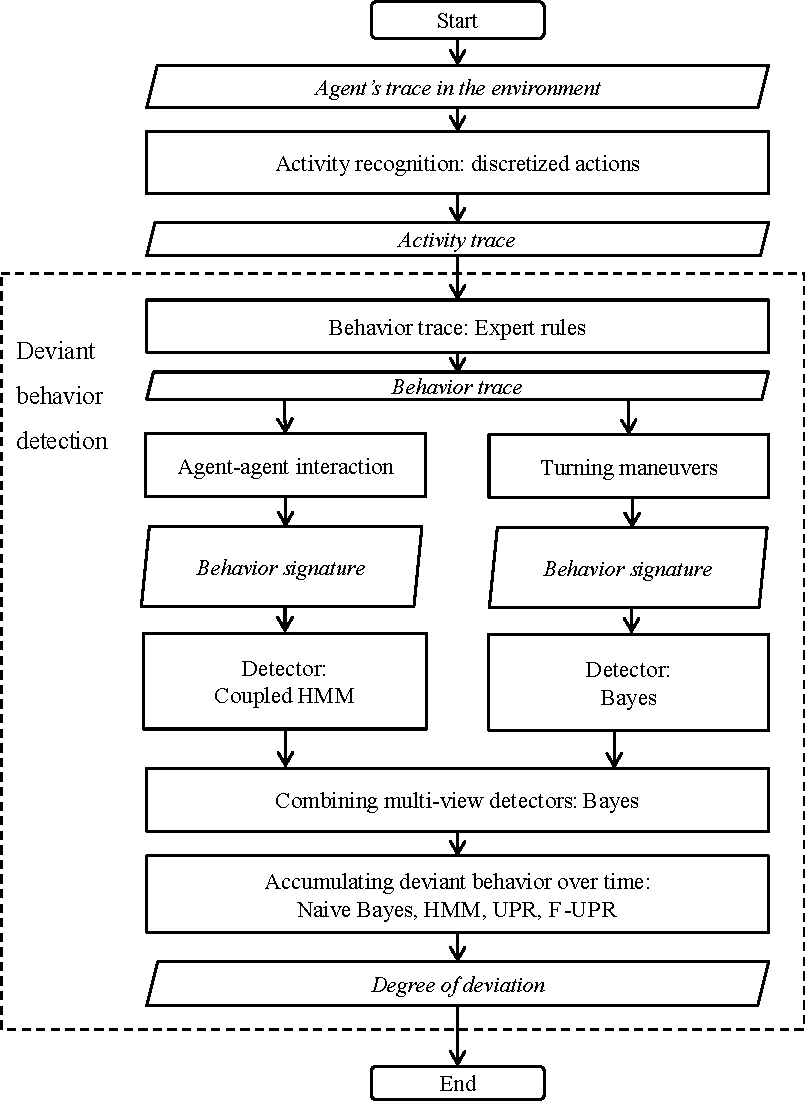
\includegraphics[width=0.8\linewidth]{chap_surveillance/stack-SURV.pdf}
\caption{Flowchart of the instantiated unified framework using two trigger event detectors and accumulating suspicious behavior.}
\label{fig:architecture-fupr}
\end{figure}


\subsection{Sensors and Observations}

The experiments in this chapter use ESCAPES~\citep{Tsai2011}, a state-of-the-art, multiagent airport evacuations simulator with several agent types exhibiting behaviors of regular travelers, authorities, and families. The agents' behavior incorporates emotional and informational interactions, such as emotional contagion, the spread of knowledge/fear, social comparison, etc. Therefore, an agent is affected other agents' emotional states, and is faced with uncertainty as to what happened and where the nearest exits are. We assume that the agent behavior corresponds to real airport passengers behavior.

ESCAPES consists of two parts: a two-dimensional environment based on the open-source project OpenSteer~\citep{opensteer}, outputting agents' physical trace coordinates; and a three-dimensional visualization component using the Massive Software~\citep{massive} to generate three-dimensional movies of the scenarios. We used a scenario that implemented the Tom Bradley International Terminal at Los Angeles International Airport, including terminals and shops as a realistic simulation environment. 

In addition to behaviors already modeled within ESCAPES, we introduced a suspicious behavior profile: an agent that behaved suspiciously prior an evacuation. Additional implementation details  are given in the experimetal section. An output example is shown in Figure~\ref{fig:airport:traces}, where traces of authorities (green), suspicious (red) and usual passengers (grey, blue) are plotted.
\begin{figure}[!ht]
\centering
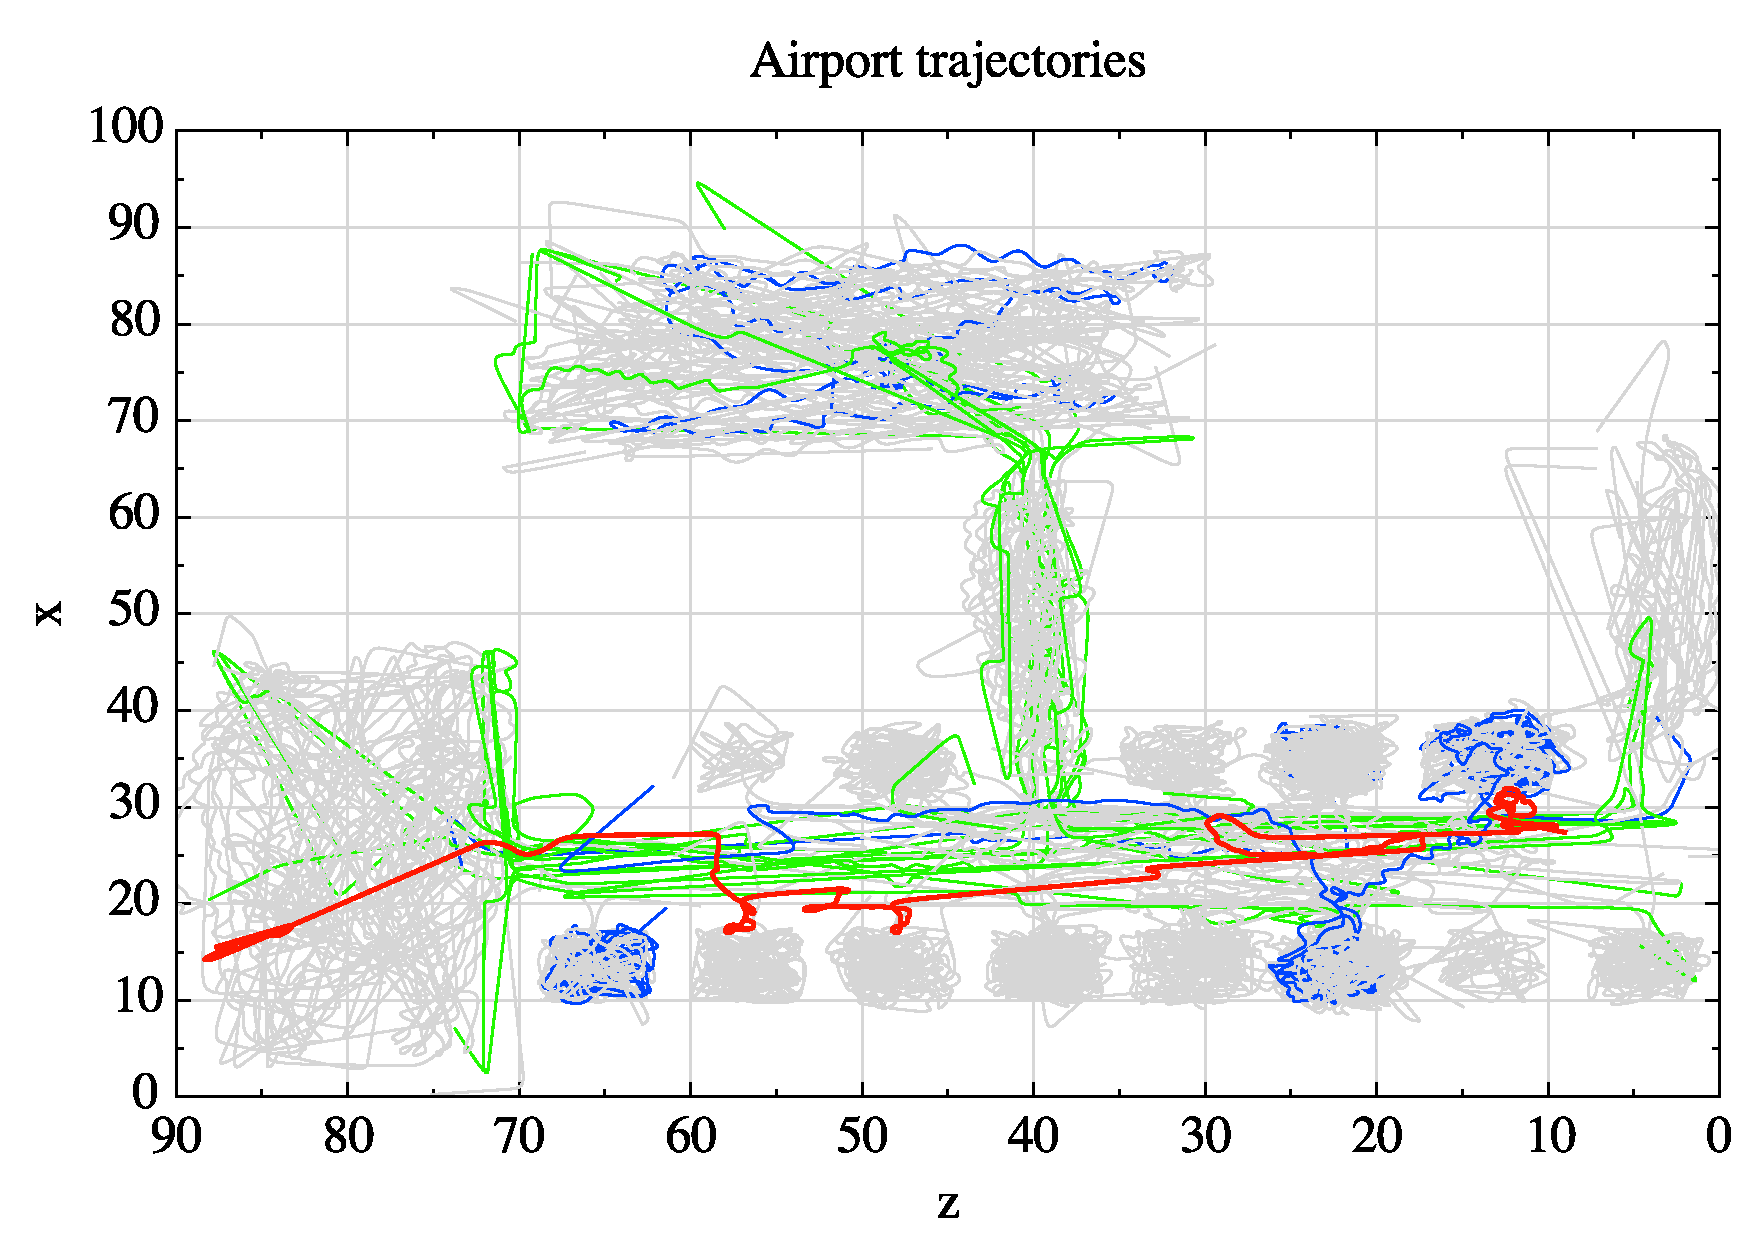
\includegraphics[width=0.95\linewidth]{chap_surveillance/airport}
\caption{Traces of all agents at the end of a simulation: authorities (green), suspicious (red), usual passengers (grey), and selected highlighted usual passengers (blue).}
\label{fig:airport:traces}
\end{figure}

An observation vector corresponds to absolute Cartesian coordinates at the airport map $\mathbf{x}_t=\tuple{x_t, y_t}$. Observation is then a sequence of vectors obtained during simulation; that is, $\mathbf{X} = \{\mathbf{x}_1, \dots, \mathbf{x}_T\}$.

%
%----------------------------------------------------------------------
%
\subsection{Atomic Activities}

%The trace of the coordinates was preprocessed to the action trace as follows. A change in position from the previous to the current state was described as taking the action of moving North, South, East and West, and their combinations (nine in total). This transformation describes the shape of a trajectory but discards the location information, which leads to better generalization. We also experimented with other transformations, for example, a more general one that also discards the orientation (forward, backward, left, right), and a less general one that divides the airport map with a square-based grid with numbered squares~\cite{Avrahami-Zilberbrand2009}. Preliminary tests showed the best performance when using the first transformation.

\index{activity recognition}
We considered three transformations of observation vectors to actions. The first divides the airport map  with a square-based grid into $N$ numbered squares~\citep{Avrahami-Zilberbrand2009}, which gives a set of possible atomic actions $\mathbb{A}_{fixed}=\{a_{s1}, \cdots, a_{sN}\}$.
Each observation sequence with Cartesian coordinates is transformed into a sequence of squares. We denote this as \emph{fixed representation}. By adjusting the square size, we can relax the model. By decreasing the square size, the model is more strict, less generalized, and may over-fit, since a too large size would cause over-generalization, that is, trajectories that are not similar might fit. %his presentation corresponds to approaches for detecting suspicious trajectories~\cite{Avrahami-Zilberbrand2009}.

The second representation, denoted as \emph{relative representation}, transforms Cartesian coordinates to actions taken in each time step as moving North, South, East, West and their combinations (nine in total); that is, 
$$\mathbb{A}_{rrep}=\{a_N, a_S, a_E, a_W, a_{NE}, a_{NW}, a_{SE}, a_{SW}, a_0\}.$$
Compared to fixed representation, relative representation also describes trajectory shape, but discards the location information, which leads to better generalization. 

The third representation, denoted as \emph{relative position and orientation}, defines actions as moving Forward, Backward, Left, Right and their combinations; that is, 
$$\mathbb{A}_{rrepor}=\{a_F, a_B, a_L, a_R, a_{FL}, a_{FR}, a_{BL}, a_{BR}, a_0\}.$$ Compared to relative representation, it also discards orientation information. 

%Preliminary tests showed 
Preliminary tests showed  the relative representation performed best \citep{Kaluza2011:PAIR}. The output of this level is an action sequence $\mathbf{a}=\{\mathbf{a}_1, \dots, \mathbf{a}_T\}$, where an action is assigned to each observation vector.


%The initialized system arch

%We address the problem of suspicious behavior detection in two steps, as shown in Figure~\ref{fig:architecture}. The first step analyzes an action trace and the surrounding environment to detect trigger events that characterize its interesting parts. The event trace then enters the second step, where it is evaluated. If the evaluation result exceeds a threshold value or is large relative to other evaluations of the event traces, then it is considered as suspicious.


%\subsection{Trigger Events}
%\label{sec:events}
%\noindent


%
%----------------------------------------------------------------------
%
\subsection{Compound Activities and Agent-Agent Interactions}

We focus on a well-known detector obtained from conversations with domain experts, and which is commonly used by behavior detection officers\footnote{An approach for monitoring passengers behavior over longer periods of time relies upon security personnel such as behavior detection officers (BDOs) that patrol airports to identify passengers who display \emph{involuntary physical and physiological actions}. US Transportation Security Administration (www.tsa.gov) trained and deployed BDO officers at over 160 US airports by 2011.}.
We observe the interactions between airport agents; more precisely, we are interested in how a passenger behaves in a uniformed authority figure's presence. A person exposed to a high level of stress produces behavior that indicates fear, anxiety, pressure, tension, deception, etc. Hence, it is rational for the suspicious agent to minimize contact with the authorities. Note, that no single avoidance is enough to raise a flag, but many such events taken together label the person as suspicious. 

We consider two types of trigger events or compound activities: interactions with authorities $\mathbb{I}=\{pass, avoid\}$, and changes of direction $\mathbb{B}=\{turn, no\_turn\}$. The idea behind these two trigger event types is to detect the likelihood that a passenger is trying to avoid an authority figure and that the change of direction occurs in general.

Both types of compound activities are detected with basic rules. The change of direction is detected by a threshold value over a trajectory curvature, while the interaction is detected by a threshold value over the distance between an authority and a passenger. The output of this level is behavior trace, where a tuple consists of a compound activity (indicating activity) and corresponding action subsequence (indicating spatial information); that is, 
$\mathbf{b}=\{\tuple{b_1, \mathbf{a}_{b_1}}, \dots, \tuple{b_{T'}, \mathbf{a}_{b_{T'}}}\}$. Such tuple is denoted \emph{trigger event} $e$, hence $\mathbf{b}=\{e_1, \dots, e_{T'}\}$.

%
%----------------------------------------------------------------------
%
\subsection{Suspicious Behavior Evaluation}

Behavior evaluation first evaluates each trigger event and estimates the likelihood that it was generated by a legitimate or a suspicious passenger, then combines the evaluations as shown in Chapter~\ref{chap:accumulation}.

The probabilities for each type of the trigger events are estimated separately. The turn event uses a \emph{frequentist estimator}; that is, \emph{a-priori} probability that a turn is generated by a suspicious or legitimate passenger:
\begin{equation}
		\hat{n}(e_t) = \Prob\{y=0|b=\text{turn}\},
\label{eq:freq-n}
\end{equation}
\begin{equation}
		\hat{s}(e_t) = \Prob\{y=1|b=\text{turn}\}.
\label{eq:freq-n}
\end{equation}

Interaction probability estimation is implemented with coupled hidden Markov models (CHMMs, introduced in Section~\ref{sec:ar:interactions}).
% %This results in a set of partial observations describing interactive behavior of a passenger. The recognition process first extracts all interactions between passengers and authority figures inside a given radius, producing a set of trajectory pairs that are transformed to relative presentation. 
%
%A trigger-event detection able to identify interactive behavior may rely on coupled hidden Markov models (CHMMs), which are briefly described below. The reader is referred to~\cite{Brand} for details; the CHMMs are not the main contribution of the paper.
% %To differentiate between authority-regular and authority-suspicious interactions we present an approach based on coupled hidden Markov models (CHMM). 
% %
The observations are constructed from two action sequences, namely the agent of interest's action sequence and the  authority agent's action sequence when they are within some predefined radius. The CHMMs use two HMM chains, where the hidden states from one chain directly impact the hidden states from the other chain. 
%Figure~\ref{fig:CHMMs} illustrates the CHMM for a pair of action traces with length $l=3$. The current state $Q_t^A$ of agent $A$ is affected by both its previous state $Q_{t-1}^A$ and previous state $Q_{t-1}^B$ of the agent $B$ (similarly $Q_t^B$ is affected by $Q_{t-1}^B$ and $Q_{t-1}^A$). Each state $Q_i$ also impacts the corresponding observation state $Y_t$. 
For example, if the authority agent moves toward the suspicious agent, the next state of the latter takes this into account and produces an action for an avoidance maneuver. 
% %The joint distribution for a pair of traces of length $k$ can be obtained by unrolling the network until we have $k$ slices, and them multiplying together all of the conditional probability distributions. 


% \begin{figure}[!ht]
% \centering
% 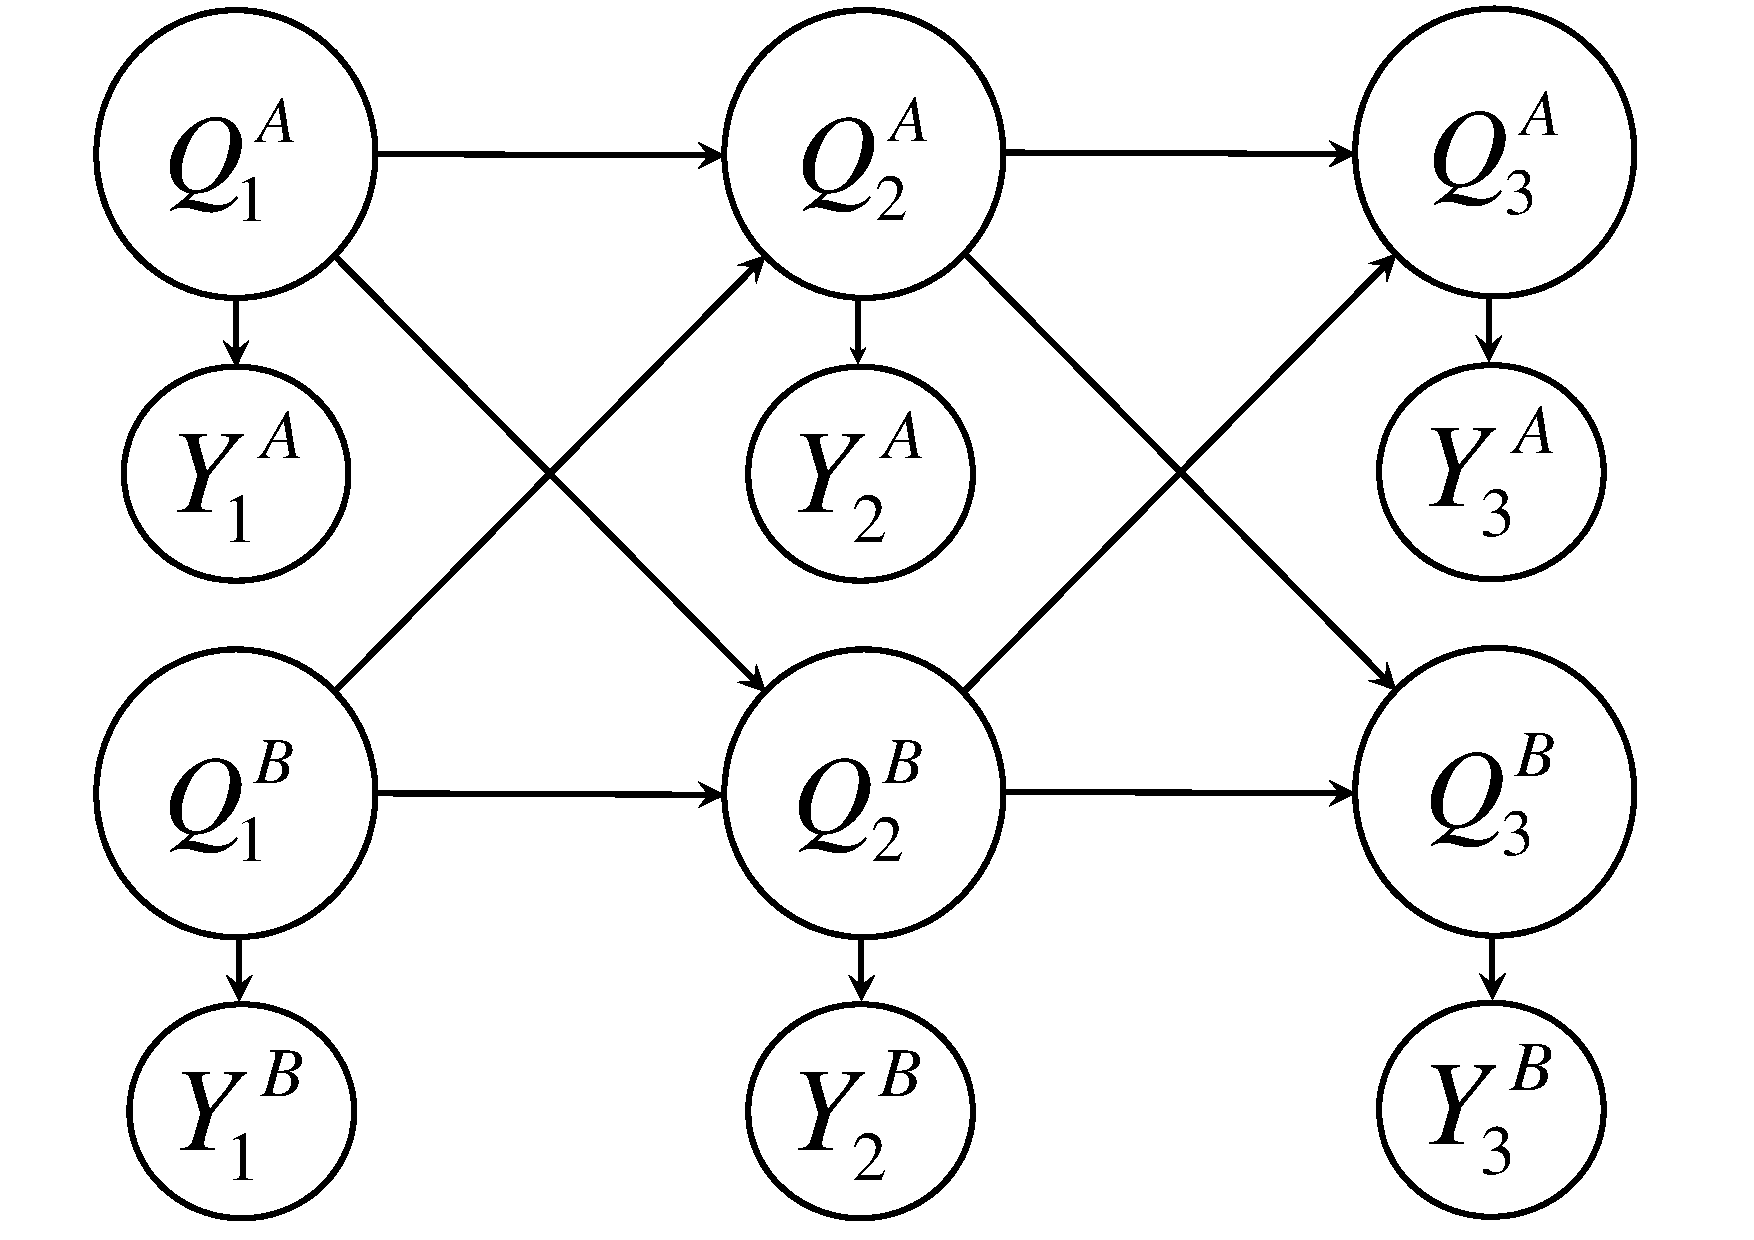
\includegraphics[bb=0 0 595 830, angle=-90, width=0.5\linewidth]{chap_surveillance/chmm.pdf}
% \caption{An example of CHMM for a pair of action traces with length $l=3$.}
% \label{fig:CHMMs}
% \end{figure}

\index{detector}
A regular passenger may not turn or do anything different in the presence of authorities, while a suspicious person will, although as described below, an observer may not be perfectly observable. Therefore, we create and train two CHMMs: $\hat{N}_I$ models authorities' and regular passengers' interactions, while $\hat{S}_I$ models authorities' and suspicious passengers' interactions. For a new event (that is, interaction) $e$, we compute the posterior probability that the event is generated with both models yielding 
\begin{equation}
		\hat{n}(e_t) = \Prob\{e|\hat{N}\},
\label{eq:freq-n}
\end{equation}
\begin{equation}
		\hat{s}(e_t) = \Prob\{e|\hat{S}\}.
\label{eq:freq-n}
\end{equation}
\noindent
We also experimented with more complex CHMM structures including other features such as relative speed and distance, but the results were comparable or even worse. 


The second step, which evaluates the trigger event sequence, uses one of the detectors introduced in Chapter~\ref{chap:accumulation}: na{\"i}ve Bayes, HMMs, UPR, and F-UPR detector.
% %As a trigger event we also extract all turns in absence of authority when the trajectory curvature exceeds a threshold value. Probabilities that a turn event was generated by suspicious $\hat{n}_T(x)$ or regular passenger $\hat{s}_T(x)$ is acquired with frequentist estimator from the learning set $D_l$.
% %
% %
% %The second architecture (Figure~\ref{fig:CHMM-3}) incorporates additional information in the form of a model of relative speed between two agents. This model directly impacts the states of both agents. The idea behind this architecture is to improve recognition results with an additional information.
% %
% %Note that for an interaction of length $T$ the architectures presented in Figure~\ref{fig:CHMMs} are unrolled to $T$ slices. %(similar as in Figure~\ref{fig:HMM-4}). 


% %\begin{figure}[!ht]
% %\centering
% %\subfigure[]{
% %\includegraphics[width=0.25\linewidth]{CHMM-2}
% %\label{fig:CHMM-2}
% %}
% %\subfigure[]{
% %\includegraphics[width=0.25\linewidth]{CHMM-3}
% %\label{fig:CHMM-3}
% %}
% %\caption{CHMM presented as 2-sliced DBN: (a) modeling actions of two agents and (b) modeling both actions and relative speed.}
% %\label{fig:CHMMs}
% %\end{figure}





%
%==========================================================================================
%
\section{Experimental Evaluation}
\label{sec:Experiments}
\noindent
In cooperation with security officials, we defined a scenario where a suspicious passenger goes from point $A$ to point $B$ while trying to avoid security personnel at the airport. One may argue that an adversary that plans to do something malicious would behave normally in the presence of authorities, and this might be true for a highly trained individual. As discussed previously, an average person exposed to a high level of stress exhibits fear, anxiety, and tension, and, hence, tries to cover it by minimizing close-range interactions by making U-turns, avoidance maneuvers, hiding in nearby shops, etc. The agent behavior implementation details within ESCAPES are provided in Appendix B.

A simulation in ESCAPES is run with a given airport map, authority agents, regular passengers, and a suspicious agent going from point $A$ to point $B$, outputting traces with 2D coordinates for all agents. 
%An example is visualized in Figure~\ref{fig:airport:traces}, where the trace of the suspicious agent is marked with red (going from left to right), traces of authorities are green and regular passengers are blue and gray.
We initialized the simulator with $100$ agents, including $K_a \in \{5,10,15,20,25\}$ authorities and a suspicious person with randomly chosen initial and final points. For each $K_a$ setting, we ran $30$ simulations, each consisting of 1,500--3,000 time steps and $100$ traces. On average, there were $215$ interactions between the authorities and the passengers per run. 
%
To avoid issues that can arise with highly unbalanced datasets, we used random re-sampling without replacement to balance the data to the ratio \textit{suspicious : normal $=20:80$}. %From the original dataset we randomly selected ${}^2/_3$ of the suspicious examples representing $20\%$ of the new dataset, and then randomly selected the matching $80\%$ from the normal examples. For each configuration we repeated the random resampling ten times and averaged the results.
For the evaluation, we used \emph{precision}, \emph{recall}, \emph{specificity} and \emph{F-measure}. 
%Precision is defined as the number of true positives (all suspicious cases correctly classified as suspicious) divided by the number of all cases marked as suspicious (true and false positives): $pr=TP/(TP+FP)$. A perfect score $1$ means that all cases marked as suspicious were indeed suspicious. Hence, the score $1-pr$ represents the rate of \emph{false alarms}. Recall is defined as the number of true positives divided by the number of all the suspicious cases: $re=TP/(TP+FN)$. A perfect score $1$ means that all the suspicious cases were detected (but says nothing about falsely marked normal cases). Similarly, the specificity is defined for normal cases $sp=TN/(TN+FP)$. There are two points of interest, depending on our objective. The first one is when both scores are minimized; that is, the trade-off point between false alarms and non-detected suspicious passengers, which can be detected with the F-measure $FM=2 \cdot pr \cdot re/(pr+re)$. The other case is when a high false-alarm rate is acceptable and non-detected cases are extremely costly. In this case we are interested in precision when recall $re=1$; that is, all the suspicious passengers are found. In the worst-case scenario, all the passengers are marked as suspicious. 
We evaluate the statistical significance of our results using the two-sample $t$-test.








\begin{figure}[!ht]
	\centering
	\subfloat[$\exists k$ rule]{\label{fig:results:rule}
		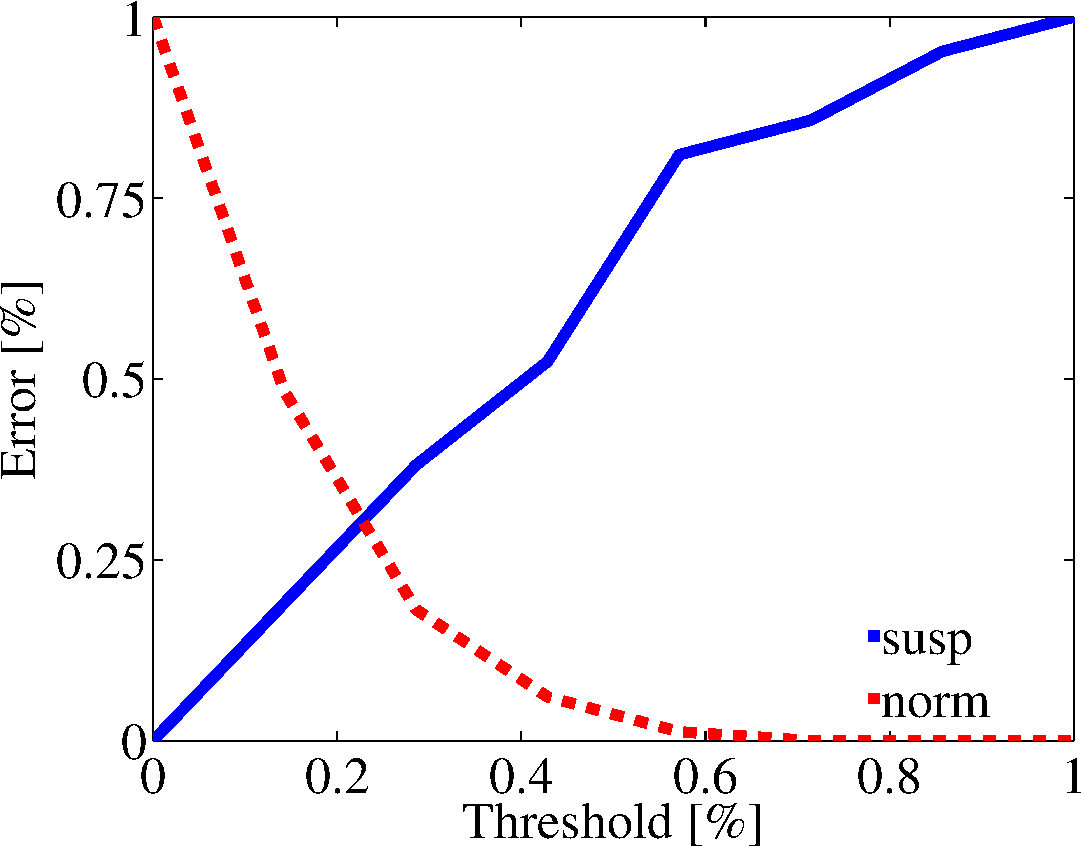
\includegraphics[width=0.45\linewidth]{chap_surveillance/k-rule}}
	\subfloat[Naive Bayes]{\label{fig:results:bayes}
		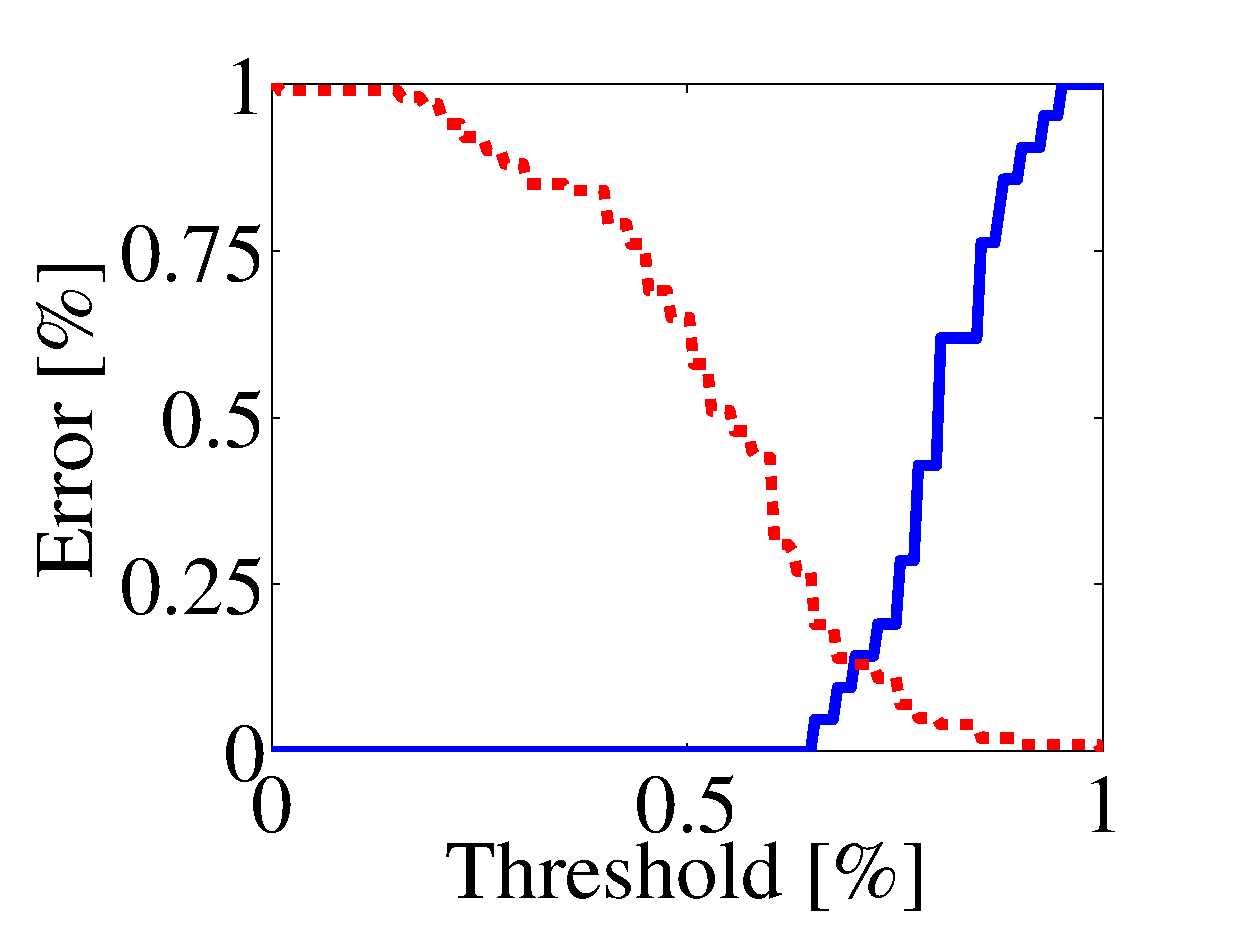
\includegraphics[width=0.45\linewidth]{chap_surveillance/bayes}}

	\subfloat[HMMs]{\label{fig:results:hmm}
		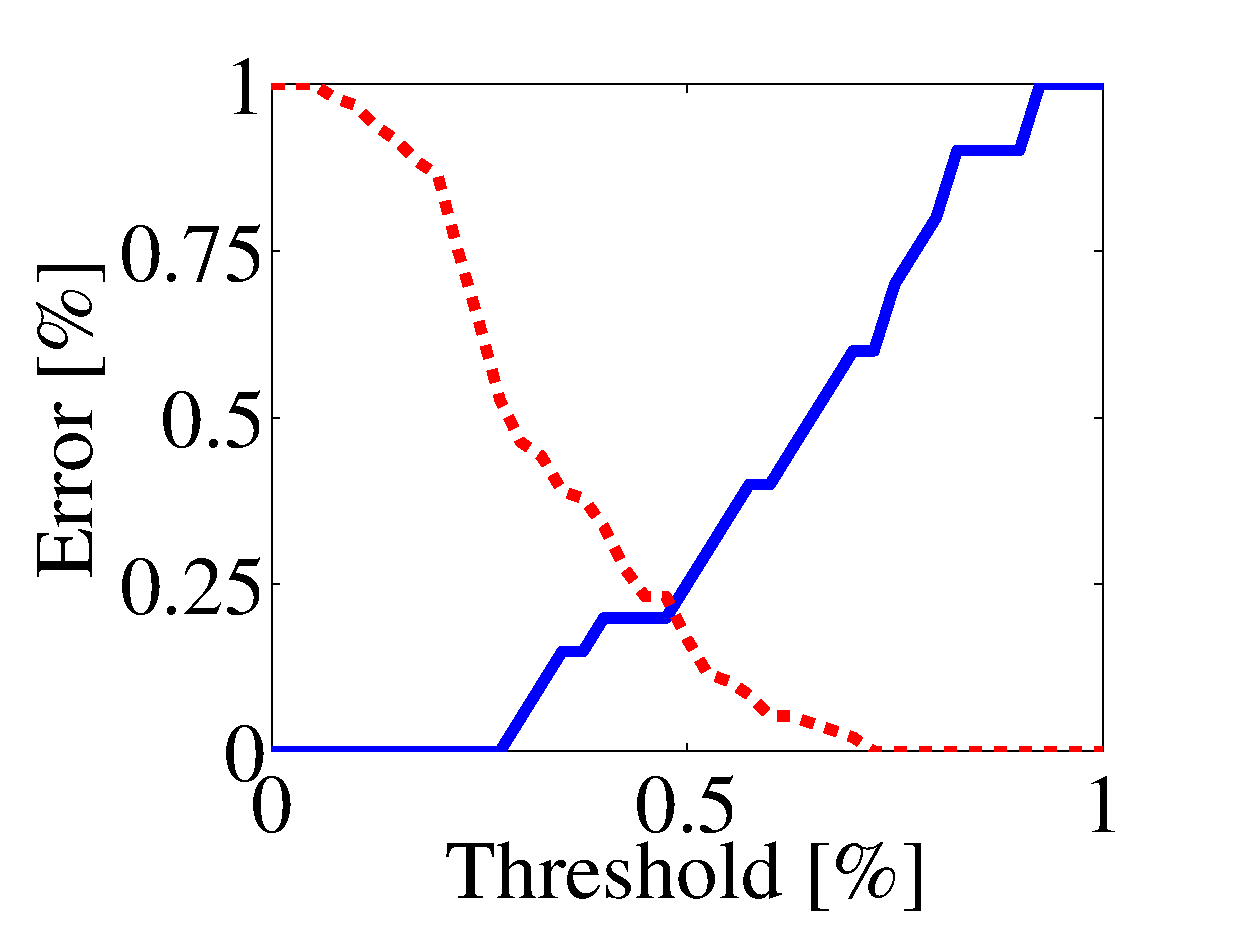
\includegraphics[width=0.45\linewidth]{chap_surveillance/hmm}}
	\subfloat[UPR]{\label{fig:results:upr}
		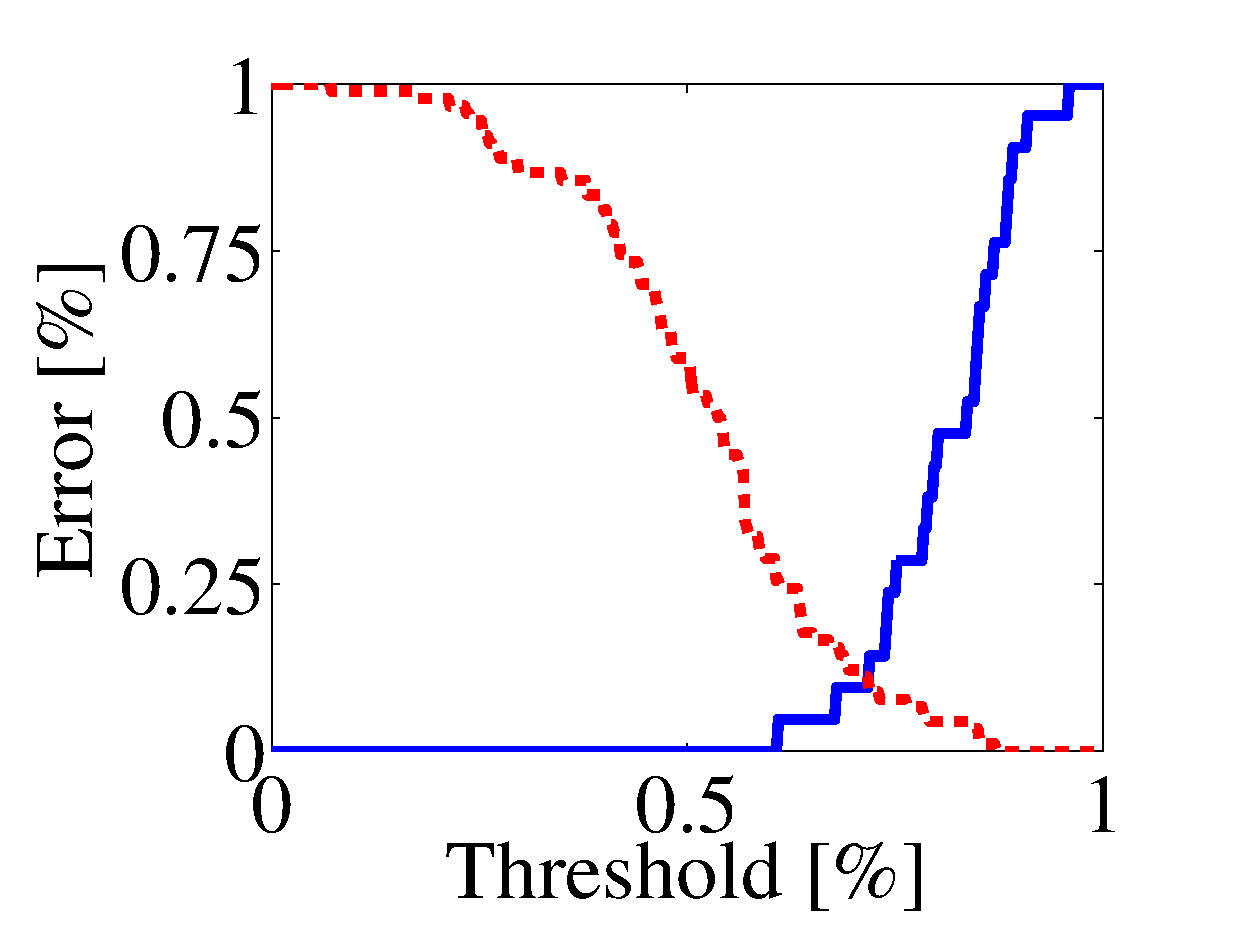
\includegraphics[width=0.45\linewidth]{chap_surveillance/upr}}

	\subfloat[F-UPR]{\label{fig:results:fupr}
		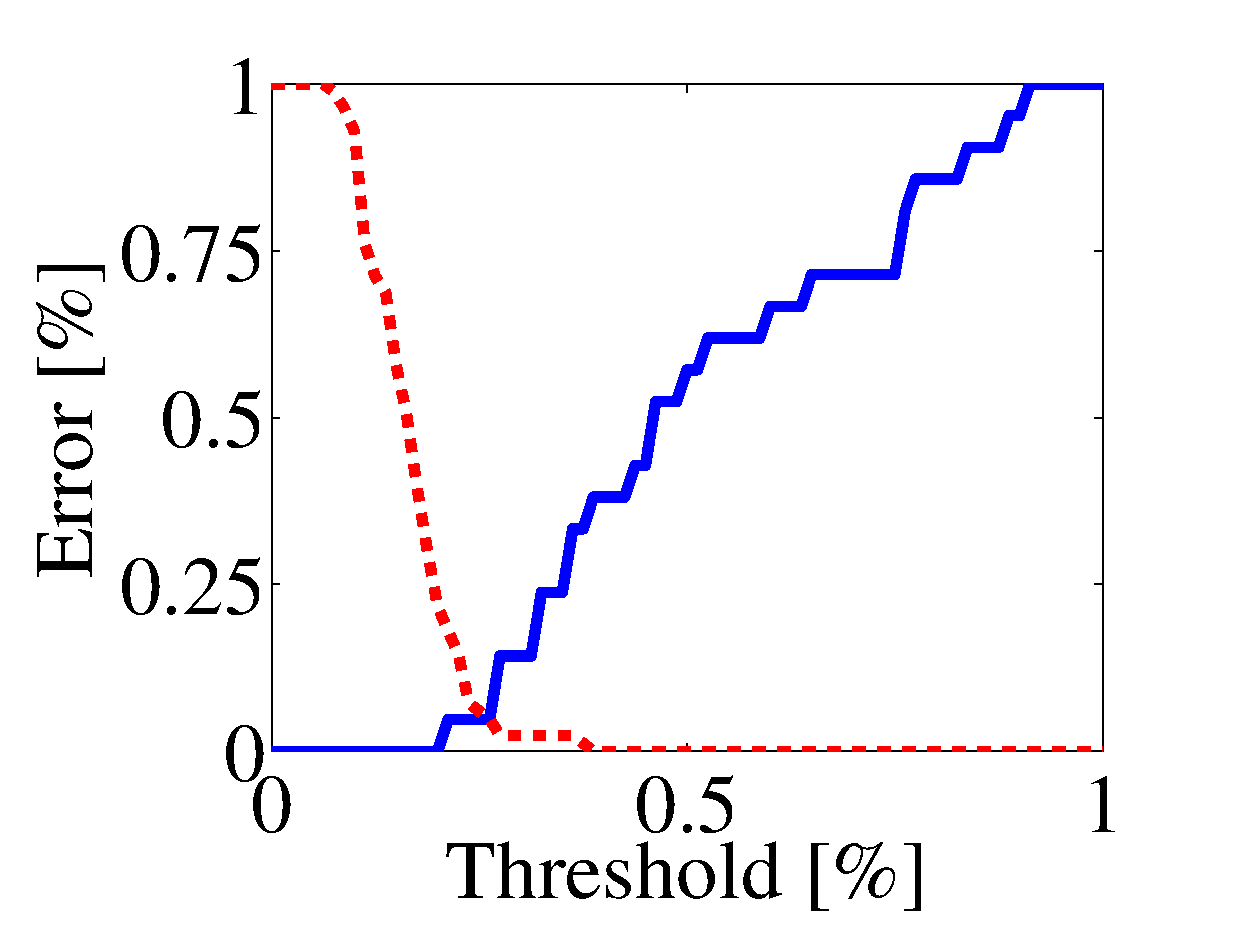
\includegraphics[width=0.45\linewidth]{chap_surveillance/espy}}

\caption{Confusion error rates for different threshold values.}
\label{fig:results}
\end{figure}






%In our case we have a two-class problem; a trace can be classified as generated either by suspicious or normal passenger. 





%TODO: comment this approach ...
%\\...
%\\...

%\subsection{Detection Based on Multiagent\\ Interactions}
%\label{sec:2Layers}
%This section compares approaches based on a two-level architecture. The first level detects trigger events, while the second level takes a trace of events and decides whether it was generated by suspicious agent. We first present the detection of trigger events based on Coupled HMMs and trajectory curvature, and then compare the discussed approaches at the second level.




%\subsubsection{Results}



%\noindent
In the first experiment, we fixed the number of authority figures $K_a=10$. We instantiated the na{\"i}ve Bayes, HMMs, UPR, and F-UPR detectors. Additionally, we considered another baseline detector using a simple rule over the threshold $k$ and the event trace $\evec{t}$, saying that if the number of suspicious events exceeds $k$ (that is, $\exists k: \eta_s(\evec{t}) > k$), then mark trace $\evec{t}$ as suspicious.
%The input to the detectors is an event trace produced by the previous level. We instantiated Naive Bayes, HMMs, UPR, and Scoring function detectors. Additionally, we consider another baseline detector using a simple rule saying that if a trace $\mathbf{x}$ contains more than $k$ events most likely generated by a suspicious passenger, then classify it a suspicious. 
%
All the detectors used the event-trace probabilities $s'(\evec{t})$ and $n'=1-s'(\evec{t})$ as returned by the event-detection step. For the HMM approach, we considered two ergodic HMMs as described in Section~\ref{sec:HMMexp}. We used two observations, the normal $\Delta(e_t)=0$ and the suspicious $\Delta(e_t)=1$ event, and varied the hidden state number. The best results were achieved with three hidden states. Note that the HMM detector applied on top of the CHMM detector basically presents a version of the mixed- layer HMM structure~\citep{Fine1998, Nguyen2005, Duong2005}. All the models, including UPR and F-UPR detectors, were evaluated with 10-fold-cross validation. %We evaluated the statistical significance of our results using two-sample $t$-test. 

Figures~\ref{fig:results}(a)--\ref{fig:results}(e) show the confusion error rates for suspicious (1-\emph{recall}) and normal (1-\emph{specificity}) passengers as a function of the normalized threshold value for all the five algorithms. For example, if the threshold is zero, then all the passengers are marked as suspicious. In this case, all the suspicious passengers are correctly identified as suspicious; hence the error rate is also zero. Also, all the normal passengers are incorrectly identified as suspicious; hence the error rate is 1. As the threshold value increases, the error rate for correctly identifying suspicious passengers increases, while the error rate for correctly identifying normal passengers decreases.

There are two points of interest: (i) when the error rates cross each other; that is, the \emph{F-measure} is maximized; and (ii) the right-most point when the error rate for suspicious passengers is zero; that is, \emph{recall}$=1$ and the false-positive rate is minimized. These cases are tabulated in Table~\ref{tab:fmeasure}. The first case is summarized in columns 2--4 showing the  recall, precision and F-measure. F-UPR outperforms the $\exists k$ rule ($p<0.01$), na{\"i}ve Bayes ($p<0.01$), HMMs ($p<0.01$), and UPR ($p<0.01$). 
{The second case, where the threshold value is such that all the suspicious passengers are discovered, is shown in columns 5 and 6. Column 5 shows the confusion error for normal passengers (that is, 1-\emph{specificity}), while column 6 shows the ratio of correctly raised alarms (that is, \emph{precision}). The $\exists k$ rule, for instance, marks all the passengers as suspicious (FP rate is $100\%$) and consequently almost $80\%$ of alarms are false. HMMs achieve better performance, but still mark more than $50\%$ of normal passengers as suspicious. Other methods mark between 1/5 and 1/4 of normal passengers as suspicious, but precision is around $50\%$, which means that every second passenger marked as suspicious is indeed suspicious (and all suspicious passengers are discovered!). Overall, F-UPR in this setting outperforms the $\exists k$ rule ($p<0.01$), na{\"i}ve Bayes ($p<0.05$), HMMs ($p<0.01$), and UPR ($p<0.05$).
Finally, Figure~\ref{fig:ROC} depicts the ROC curves showing that F-UPR performs the same, or better, in all the threshold settings. 

\begin{figure}[!ht]
\centering
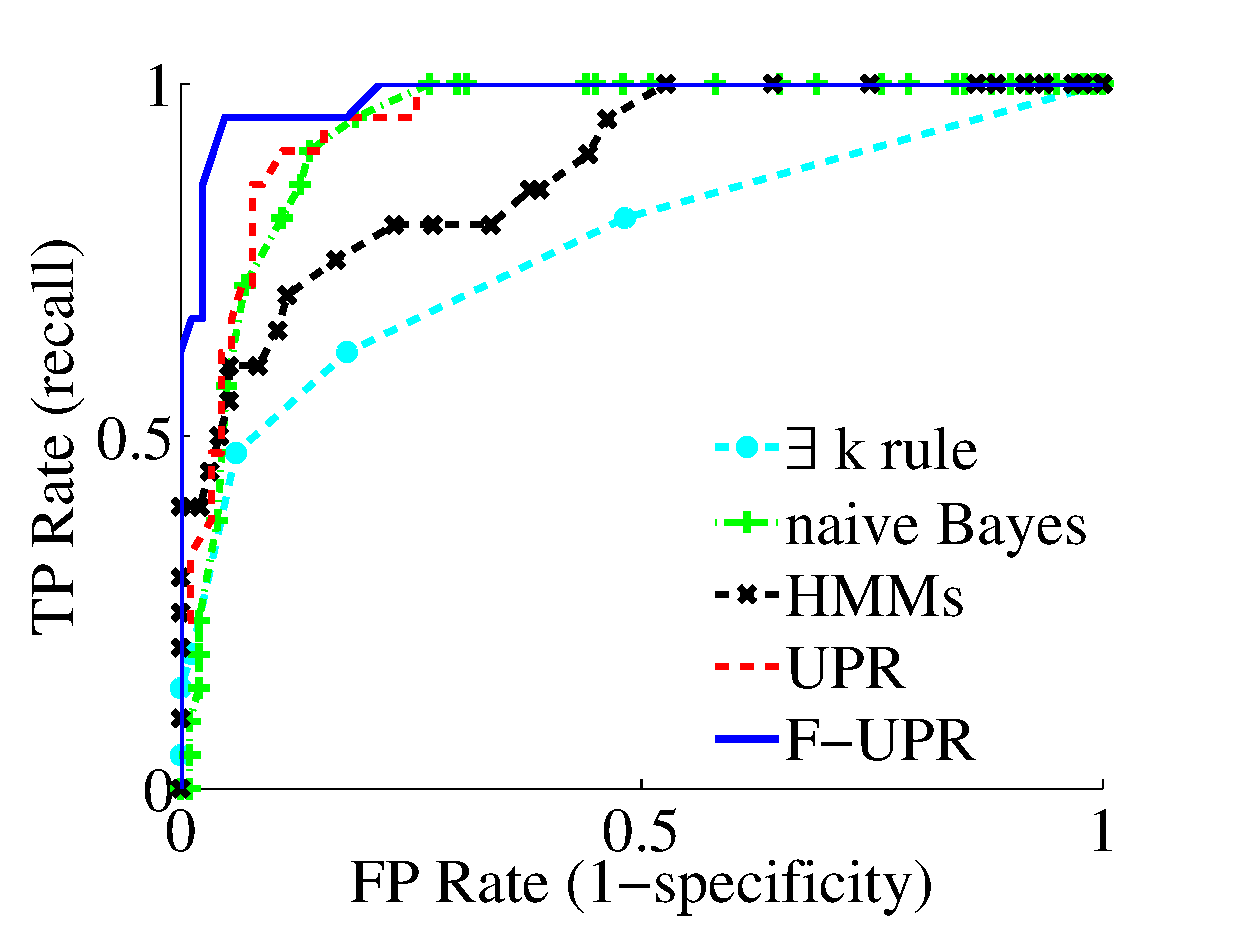
\includegraphics[width=0.8\linewidth]{chap_surveillance/ROC}
\caption{ROC curves comparing all the detectors.}
\label{fig:ROC}
\end{figure}

\begin{table}
\centering
\caption{Evaluation results when the F-measure is maximized (columns 2--4) and all the suspicious cases are discovered (the last two columns).}
\renewcommand{\arraystretch}{1.2}
\begin{tabular}{c|ccc|cc}
	\hline
						&	\multicolumn{3}{c|}{maximized F-measure}		&	\multicolumn{2}{c}{$recall$=1}		\\
	\hline
		Algorithm					& $re$	& $pr$	& $FM$		& $1-spec$		& $pr$\\		
	\hline
	$\exists k$ rule		& 0.619		& 0.464		& 0.530		& 1.000		& 0.202		\\		
	Naive Bayes				& 0.857		& 0.581		& 0.693		& 0.270		& 0.436		\\
	HMMs						& 0.600		& 0.706		& 0.649		& 0.526		& 0.286		\\
	UPR						& 0.857		& 0.720		& 0.783		& 0.256		& 0.477		\\
	F-UPR						& 0.905		& 0.905		& 0.905		& 0.217		& 0.539		\\
	\hline
\end{tabular}
\label{tab:fmeasure}
\end{table}

%\begin{table}
%\centering
%\caption{False positive and false negative rate when all suspicious cases are discovered ($re=1$).}
%\renewcommand{\arraystretch}{1.2}
%\begin{tabular}{c|c|c}
%	\hline
%		Algorithm			&FP rate ($1 - spec$)	 & Precision\\		
%	\hline
%	$\exists k$ rule		& 1.000		&0.202		\\		
%	Naive Bayes				& 0.270		&0.436 		\\
%	HMMs						& 0.526		&0.286	\\
%	UPR						& 0.256		&0.477	\\
%	F-UPR						& 0.217		&0.539	\\
%	\hline
%\end{tabular}
%\label{tab:getall}
%\end{table}


\begin{figure}[!ht]
\centering
\subfloat[F-measure is maximized.]{
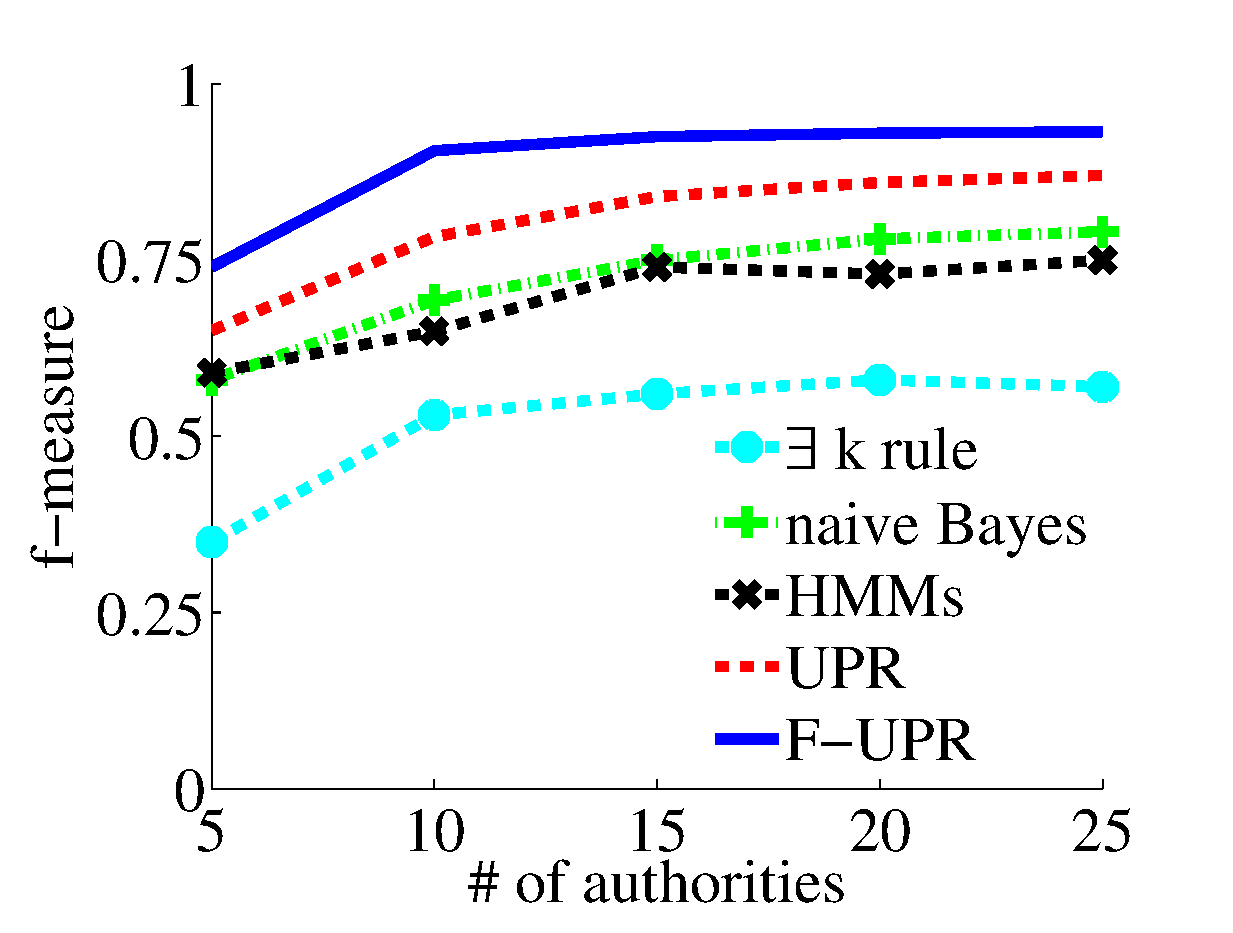
\includegraphics[width=0.6\linewidth]{chap_surveillance/authvar-fm}
\label{fig:authvar:fmeasure}
}

\subfloat[All suspicious passengers are discovered.]{
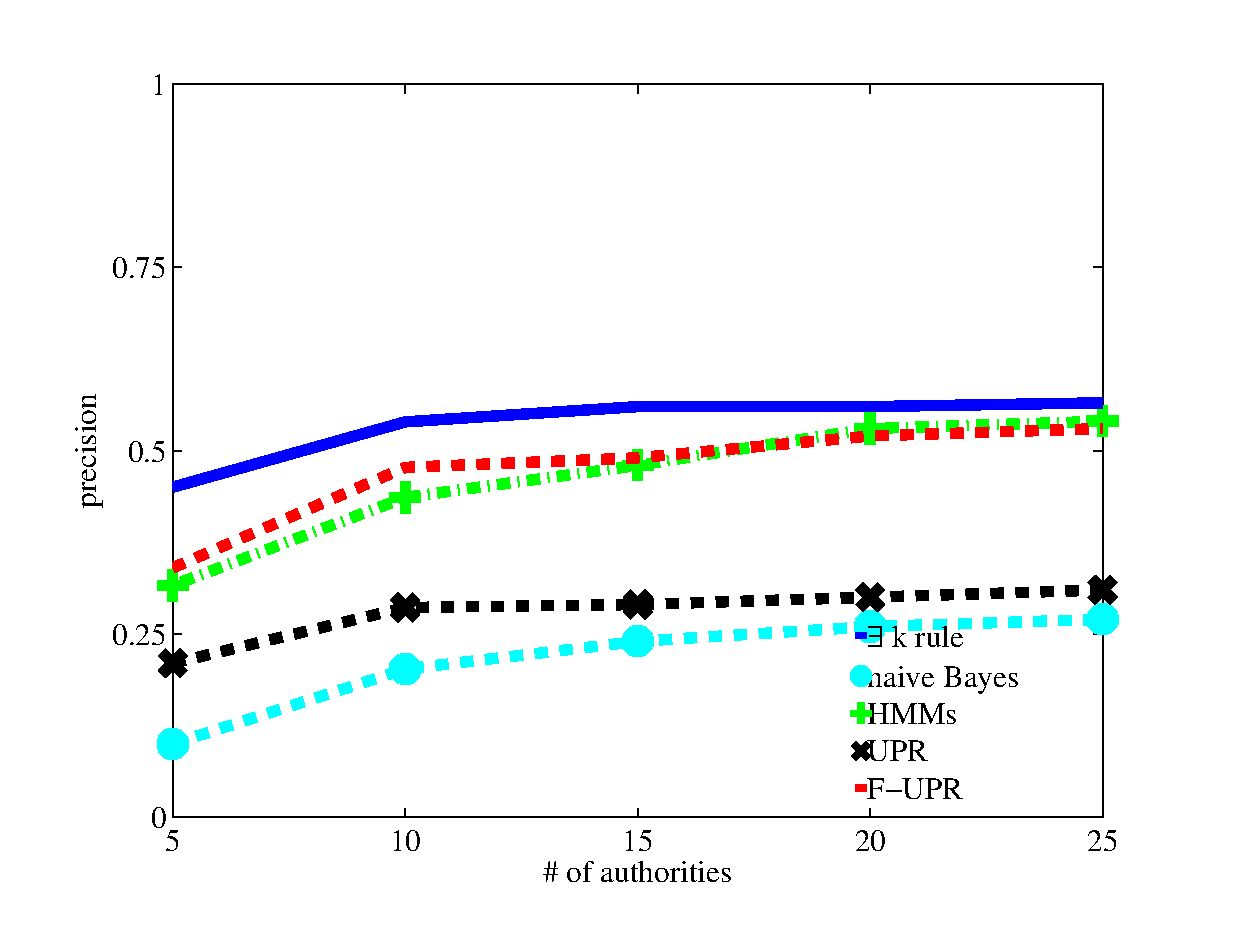
\includegraphics[width=0.6\linewidth]{chap_surveillance/authvar-pr}
\label{fig:authvar:precision}
}
\caption{Evaluation results for varying the authority figure number in the simulation and two different threshold values.}
\label{fig:authvar}
\end{figure}

In the last experiment, we varied the number of simulated authorities. We expected that increased authority figures will result in more interactions with suspicious passengers, making detection easier. Figure~\ref{fig:authvar} shows the results for the $K_a \in \{5,10,15,20,25\}$ authority figures in a simulation:  Figure~\ref{fig:authvar:fmeasure} shows the F-measure for a maximizing threshold, while Figure~\ref{fig:authvar:precision} shows the precision when $\text{recall}=1$. Increased authority figures significantly increases detection capabilities. For example, the F-measure for F-UPR increases by $15\%$ when the security resources are doubled from five to ten, but as the number increases, the impact is smaller. We can also see that F-UPR achieves the same performance as other methods using significantly fewer security resources. 
%



\subsection{Detection Based on the Action Sequence}
\label{sec:HMMexp}
\noindent
We also applied a sanity check and tested the suspicious behavior detection from a sequence of agent actions (that is, action sequence $\mathbf{a}$) instead of a sequence of trigger events (that is, event trace $\mathbf{e}$). We used HMMs, since they are considered a baseline for modeling action sequences. The goal is to differentiate between a sequence produced by a suspicious and by a regular passenger. We expect this approach to perform poorly, since it is too general to precisely model interactive behavior present in a multiagent environment.

The suspicious behavior detector consists of two ergodic HMMs: $S'$ trained on the suspicious traces and $N'$ trained on the regular action traces. A new trace is first transformed to the action trace $\avec{k}$ as previously described and then matched against both HMMs, yielding the likelihood that it produced the given $\avec{k}$. If the likelihood is greater than a threshold, the action trace is marked as suspicious. 
%
%, and normal otherwise.%a behavior produced by the most probable model.%: $argmax(H_s(r), H_n(r))$.
%$$\frac{\lambda' \Prob\{ \avec{k}|S'\}}{(\lambda'}\Prob\{ \avec{k}|S'\} + (1-\check{\lambda})\Prob\{ \mathbf{x}|\check{N}\})} > \check{\tau},$$
%We run the experiments on We experimented with different number of hidden states and the best results are summarized in Table~\ref{}.
%We first report the results of running single-level HMMs with three different state presentations. 
%Table~\ref{tab:HMMresults} shows recall, precision and F-measure for trajectories presented with absolute position (column 2), relative position (column 3), and relative position and orientation (column 4). The second row shows results with acceptable discovery rate (recall), but extremely low precision around $10\%$ in the third row. This means that only $1$ out of $10$ passengers marked as suspicious was indeed suspicious. States presented with relative position outperform presentations with absolute position, which was expected. Absolute position requires a large data set to cover the complete state space, and second, it is prone to over-fitting. The presentations with relative position and orientation achieved lower recall than other presentations and slightly better precision. The reason can be in over-generalization. However, states represented with relative position were used in further experiments. 
%
We tested this approach for $K_a=10$ authorities. At the threshold value such that the highest F-measure 18.01 was achieved, this approach achieved an acceptable discovery rate ($\text{recall}=66.23$) and an extremely low precision (10.42). Such a performance positions this approach under the $\exists k$ rule.  The overall performance was consistent with our expectation that modeling single-agent actions in a multiagent environment would not capture the interactive behavior. 

%\begin{table}
%\centering
%\caption{Evaluation results for HMMs applied to the whole sequence of 2D coordinates presented as actions.}
%\renewcommand{\arraystretch}{1.2}
%\begin{tabular}{c|ccc}
%	\hline
%		[\%]		& Abs. pos.	& Rel. pos.	& Rel. pos.\&ori.\\		
%	\hline
%	Recall		& 62.63		& 66.23		& 40.86 		\\		
%	Precision	& 7.04		& 10.42		& 11.54 		\\
%	F-measure	& 13.24		& 18.01		& 18.00 		\\
%	\hline
%\end{tabular}
%\label{tab:HMMresults}
%\end{table}




\section{Identifying a Dangerous Driver}
\noindent
In addition to the airport domain, we applied UPR and F-UPR to the dangerous-driver domain, as introduced in \cite{Avrahami-Zilberbrand2009}. This domain also includes behavior that becomes increasingly costly if repeated: a driver switching a lane once or twice is not necessarily acting suspiciously, but a driver zigzagging across two lanes is dangerous. Our goal was to detect such drivers as soon as possible. 
%An example shown in Figure~\ref{fig:driver} depicts two lanes divided by a gird. There are two straight trajectories and one zigzag trajectory from left to right lane. 
%From each position, the driver can move horizontally to the next cell in the row, or to one of the diagonal cells.  A car in the left lane may be mistakenly observed (with small probability) to be in the right lane, and vice versa.

%\begin{figure}[h]
%\centering
%\includegraphics[width=0.7\textwidth, bb=0 0 1170 355]{lanes.pdf}
%\caption{Simulated trajectories for drivers~\cite{Avrahami-Zilberbrand2009}.}
%\label{fig:driver}
%\end{figure}

We generated 100 zigzagging driver observation sequences, each consisting of N observations, and 1,000 safe driver sequences. The trajectory observations were sampled with 10\% noise. If the driver stayed on the same lane as in the previous sample, the event was considered normal; otherwise, it was considered dangerous. For each sequence of trigger events, we accumulated the associated cost using both UPR and F-UPR. 
%Depending on a chosen threshold value, a driver may be declared dangerous if its accumulated cost is greater than the threshold, and safe if its accumulated cost is smaller than the threshold. 
Due to observation noise, the task is expected to be more difficult when less observations are available. As the number of available observations increases, it should be easier to distinguish between safe and dangerous drivers.


Table~\ref{tab:zigzag} reports the performance at the peak F-measure for different observation sequence lengths. The results confirm the airport domain experiments for two points. First, F-UPR performs better than UPR for any selected sequence length. Second, the performance of both methods increases as the number of observations increases, where F-UPR requires fewer observations than UPR to achieve the same performance. 
%Figure~\ref{fig:error} shows the confusion error rates at $N=75$, while Figure~\ref{fig:roc} compares ROC curves at the same observation sequence length. Figures for other $N$ values are quite similar and hence omitted.


\begin{table}[]
\centering
\caption{Evaluation results at the peak F-measure in the dangerous driver domain.}
\begin{tabular}{ccc}
\toprule
	Sequence length $N$ & F-UPR & UPR	\\
	\hline
	25 	&	0.632	&	0.540	\\
	50 	&	0.720	&	0.667	\\
	75 	&	0.900	&	0.800	\\
	100 &	0.952	&	0.857	\\
	125 &	1.000	&	0.947	\\
\toprule
\end{tabular}
\label{tab:zigzag}
\end{table}


\section{Conclusion}
\label{sec:Conclusion}
\noindent
This chapter instantiated the unified detection framework to successfully address the problem of suspicious behavior detection from a set of observations, where no single observation suffices to make the decision. The chapter addressed the problem in two steps; that is, the trigger event detection and a combination of evidence to reach a final conclusion. The proposed F-UPR approach was compared to competing approaches with comprehensive experiments on two simulated domains.
%a simulated airport domain. 
%By providing a new algorithm that outperforms other approaches, this paper has advanced the state of the art.




%We have modeled a trace of multiple trigger events as a mixture of two stochastic processes, normal and suspicious. We have defined detection of suspicious behavior as identifying those traces generated by the suspicious process. We have shown that optimal detection must take into account the complete history in the trace, which present a challenge in real-world applications. We discuss approaches that simplify detection by estimating conditional probabilities as well as approaches that relay on other frameworks such as plan recognition. We proposed a heuristic approach based on a family of \emph{well-behaved} scoring functions that interpret event to produce a score presenting overall suspicion that the trace corresponds to behavior of the suspicious agent using the complete behavior of the agent in the past. The approach was compared on the airport domain against both trajectory-based detection using HMMs and event-based detection using CHMM for detecting events and Naive Bayes, HMMs, UPR, and rule baseline for evaluating event traces. All of them were outperformed by the proposed approach.

%Verification procedure\\
% - evaluation on motivating domain -- airport scenario\\
% - proposes event detection procedure\\
% - compare different approaches using simulation
%Experimental evaluation on the airport domain first proposes an approach for detecting trigger events and then compares discussed approaches for evaluating whether an event trace is generated by normal or suspicious agent against the heuristic approach. The experiments in simulated multiagent environment show that the proposed approach outperforms other discussed solutions.


%TODO: UPDATE \emph{The paper presented EPSY, an event-based keyhole detector of suspicious behavior based on evaluating multiple partial observations by incorporating four key features: (i) dealing with infrequent partial observations; (ii) incorporating uncertainty arising from keyhole approach; (iii) forgetting mechanism; and (iv) adaptive reward and penalty functions. The approach was demonstrated on a motivating domain showing that ESPY is significantly better than basic, single-layered HMMs and two-layered HLHMMs, and comparable to the UPR approach. However, the ESPY showed that it can provide a viable solution for the detection of suspicious behavior by evaluating partial observations. It should be noted that the originality of this approach is inherent in the adaptive evaluation of multiple partial observations related to the behavior of an agent in the past. 
%
%An interesting perspective for the enrichment of the ESPY consists in active detection of erratic behavior by intentionally provoking responses from an agent for which there is either unclear or not enough information to draw the conclusion.}

With automatic behavior surveillance is it possible to identify passengers showing suspicious behavior that currently remains unnoticed. However, there are still shortcomings that are hard to bypass. For instance, observers can perceive whether someone appears anxious or is acting deceptively, they cannot tell whether that person is planning an attack or an extramarital affair. Although the \emph{intelligent behavioral surveillance} presents an important leap in security, it raises several privacy violation concerns, which should be addressed before deploying such systems in practice.



%In many cases, the extra scrutiny is a casual conversation with a TSA behavior officer that shows someone is innocent, 

%"behavioral surveillance" has "enormous potential for violating" privacy.

%"The shortcoming is, we don't know how many people are showing suspicious behaviors and aren't being noticed," Ekman said.

%Although observers can perceive whether someone appears anxious or is acting deceptively, they can't tell whether that person is planning an attack or something such as an extramarital affair, Levenson said.

%Our goal is to monitor a passenger 

%Airport security has increased drastically in recent years.
%Nowadays the security at the airports 
%Motivation...


%ACKNOWLEDGMENTS are optional
%\section{Acknowledgments}
%The authors would like to thank Zhengyu Yin for valuable discussion and suggestions, and Jason Tsai and Matthew Brown for their help with implementation challenges in the ESCAPES simulator. The work of Bo{\v s}tjan Kalu{\v z}a was supported partly by the Slovene Human Resources Development and Scholarship Fund and partly by the Slovenian Research Agency.
